% Options for packages loaded elsewhere
\PassOptionsToPackage{unicode}{hyperref}
\PassOptionsToPackage{hyphens}{url}
%
\documentclass[
  doc,12pt,floatsintext]{apa7}
\usepackage{amsmath,amssymb}
\usepackage{iftex}
\ifPDFTeX
  \usepackage[T1]{fontenc}
  \usepackage[utf8]{inputenc}
  \usepackage{textcomp} % provide euro and other symbols
\else % if luatex or xetex
  \usepackage{unicode-math} % this also loads fontspec
  \defaultfontfeatures{Scale=MatchLowercase}
  \defaultfontfeatures[\rmfamily]{Ligatures=TeX,Scale=1}
\fi
\usepackage{lmodern}
\ifPDFTeX\else
  % xetex/luatex font selection
  \setmainfont[]{Times New Roman}
\fi
% Use upquote if available, for straight quotes in verbatim environments
\IfFileExists{upquote.sty}{\usepackage{upquote}}{}
\IfFileExists{microtype.sty}{% use microtype if available
  \usepackage[]{microtype}
  \UseMicrotypeSet[protrusion]{basicmath} % disable protrusion for tt fonts
}{}
\makeatletter
\@ifundefined{KOMAClassName}{% if non-KOMA class
  \IfFileExists{parskip.sty}{%
    \usepackage{parskip}
  }{% else
    \setlength{\parindent}{0pt}
    \setlength{\parskip}{6pt plus 2pt minus 1pt}}
}{% if KOMA class
  \KOMAoptions{parskip=half}}
\makeatother
\usepackage{xcolor}
\usepackage{color}
\usepackage{fancyvrb}
\newcommand{\VerbBar}{|}
\newcommand{\VERB}{\Verb[commandchars=\\\{\}]}
\DefineVerbatimEnvironment{Highlighting}{Verbatim}{commandchars=\\\{\}}
% Add ',fontsize=\small' for more characters per line
\usepackage{framed}
\definecolor{shadecolor}{RGB}{248,248,248}
\newenvironment{Shaded}{\begin{snugshade}}{\end{snugshade}}
\newcommand{\AlertTok}[1]{\textcolor[rgb]{0.94,0.16,0.16}{#1}}
\newcommand{\AnnotationTok}[1]{\textcolor[rgb]{0.56,0.35,0.01}{\textbf{\textit{#1}}}}
\newcommand{\AttributeTok}[1]{\textcolor[rgb]{0.13,0.29,0.53}{#1}}
\newcommand{\BaseNTok}[1]{\textcolor[rgb]{0.00,0.00,0.81}{#1}}
\newcommand{\BuiltInTok}[1]{#1}
\newcommand{\CharTok}[1]{\textcolor[rgb]{0.31,0.60,0.02}{#1}}
\newcommand{\CommentTok}[1]{\textcolor[rgb]{0.56,0.35,0.01}{\textit{#1}}}
\newcommand{\CommentVarTok}[1]{\textcolor[rgb]{0.56,0.35,0.01}{\textbf{\textit{#1}}}}
\newcommand{\ConstantTok}[1]{\textcolor[rgb]{0.56,0.35,0.01}{#1}}
\newcommand{\ControlFlowTok}[1]{\textcolor[rgb]{0.13,0.29,0.53}{\textbf{#1}}}
\newcommand{\DataTypeTok}[1]{\textcolor[rgb]{0.13,0.29,0.53}{#1}}
\newcommand{\DecValTok}[1]{\textcolor[rgb]{0.00,0.00,0.81}{#1}}
\newcommand{\DocumentationTok}[1]{\textcolor[rgb]{0.56,0.35,0.01}{\textbf{\textit{#1}}}}
\newcommand{\ErrorTok}[1]{\textcolor[rgb]{0.64,0.00,0.00}{\textbf{#1}}}
\newcommand{\ExtensionTok}[1]{#1}
\newcommand{\FloatTok}[1]{\textcolor[rgb]{0.00,0.00,0.81}{#1}}
\newcommand{\FunctionTok}[1]{\textcolor[rgb]{0.13,0.29,0.53}{\textbf{#1}}}
\newcommand{\ImportTok}[1]{#1}
\newcommand{\InformationTok}[1]{\textcolor[rgb]{0.56,0.35,0.01}{\textbf{\textit{#1}}}}
\newcommand{\KeywordTok}[1]{\textcolor[rgb]{0.13,0.29,0.53}{\textbf{#1}}}
\newcommand{\NormalTok}[1]{#1}
\newcommand{\OperatorTok}[1]{\textcolor[rgb]{0.81,0.36,0.00}{\textbf{#1}}}
\newcommand{\OtherTok}[1]{\textcolor[rgb]{0.56,0.35,0.01}{#1}}
\newcommand{\PreprocessorTok}[1]{\textcolor[rgb]{0.56,0.35,0.01}{\textit{#1}}}
\newcommand{\RegionMarkerTok}[1]{#1}
\newcommand{\SpecialCharTok}[1]{\textcolor[rgb]{0.81,0.36,0.00}{\textbf{#1}}}
\newcommand{\SpecialStringTok}[1]{\textcolor[rgb]{0.31,0.60,0.02}{#1}}
\newcommand{\StringTok}[1]{\textcolor[rgb]{0.31,0.60,0.02}{#1}}
\newcommand{\VariableTok}[1]{\textcolor[rgb]{0.00,0.00,0.00}{#1}}
\newcommand{\VerbatimStringTok}[1]{\textcolor[rgb]{0.31,0.60,0.02}{#1}}
\newcommand{\WarningTok}[1]{\textcolor[rgb]{0.56,0.35,0.01}{\textbf{\textit{#1}}}}
\usepackage{graphicx}
\makeatletter
\def\maxwidth{\ifdim\Gin@nat@width>\linewidth\linewidth\else\Gin@nat@width\fi}
\def\maxheight{\ifdim\Gin@nat@height>\textheight\textheight\else\Gin@nat@height\fi}
\makeatother
% Scale images if necessary, so that they will not overflow the page
% margins by default, and it is still possible to overwrite the defaults
% using explicit options in \includegraphics[width, height, ...]{}
\setkeys{Gin}{width=\maxwidth,height=\maxheight,keepaspectratio}
% Set default figure placement to htbp
\makeatletter
\def\fps@figure{htbp}
\makeatother
\setlength{\emergencystretch}{3em} % prevent overfull lines
\providecommand{\tightlist}{%
  \setlength{\itemsep}{0pt}\setlength{\parskip}{0pt}}
\setcounter{secnumdepth}{5}
% Make \paragraph and \subparagraph free-standing
\ifx\paragraph\undefined\else
  \let\oldparagraph\paragraph
  \renewcommand{\paragraph}[1]{\oldparagraph{#1}\mbox{}}
\fi
\ifx\subparagraph\undefined\else
  \let\oldsubparagraph\subparagraph
  \renewcommand{\subparagraph}[1]{\oldsubparagraph{#1}\mbox{}}
\fi
% definitions for citeproc citations
\NewDocumentCommand\citeproctext{}{}
\NewDocumentCommand\citeproc{mm}{%
  \begingroup\def\citeproctext{#2}\cite{#1}\endgroup}
\makeatletter
 % allow citations to break across lines
 \let\@cite@ofmt\@firstofone
 % avoid brackets around text for \cite:
 \def\@biblabel#1{}
 \def\@cite#1#2{{#1\if@tempswa , #2\fi}}
\makeatother
\newlength{\cslhangindent}
\setlength{\cslhangindent}{1.5em}
\newlength{\csllabelwidth}
\setlength{\csllabelwidth}{3em}
\newenvironment{CSLReferences}[2] % #1 hanging-indent, #2 entry-spacing
 {\begin{list}{}{%
  \setlength{\itemindent}{0pt}
  \setlength{\leftmargin}{0pt}
  \setlength{\parsep}{0pt}
  % turn on hanging indent if param 1 is 1
  \ifodd #1
   \setlength{\leftmargin}{\cslhangindent}
   \setlength{\itemindent}{-1\cslhangindent}
  \fi
  % set entry spacing
  \setlength{\itemsep}{#2\baselineskip}}}
 {\end{list}}
\usepackage{calc}
\newcommand{\CSLBlock}[1]{\hfill\break\parbox[t]{\linewidth}{\strut\ignorespaces#1\strut}}
\newcommand{\CSLLeftMargin}[1]{\parbox[t]{\csllabelwidth}{\strut#1\strut}}
\newcommand{\CSLRightInline}[1]{\parbox[t]{\linewidth - \csllabelwidth}{\strut#1\strut}}
\newcommand{\CSLIndent}[1]{\hspace{\cslhangindent}#1}
\ifLuaTeX
\usepackage[bidi=basic]{babel}
\else
\usepackage[bidi=default]{babel}
\fi
\babelprovide[main,import]{english}
\ifPDFTeX
\else
\babelfont{rm}[]{Times New Roman}
\fi
% get rid of language-specific shorthands (see #6817):
\let\LanguageShortHands\languageshorthands
\def\languageshorthands#1{}
% Manuscript styling
\usepackage{upgreek}
\captionsetup{font=singlespacing,justification=justified}

% Table formatting
\usepackage{longtable}
\usepackage{lscape}
% \usepackage[counterclockwise]{rotating}   % Landscape page setup for large tables
\usepackage{multirow}		% Table styling
\usepackage{tabularx}		% Control Column width
\usepackage[flushleft]{threeparttable}	% Allows for three part tables with a specified notes section
\usepackage{threeparttablex}            % Lets threeparttable work with longtable

% Create new environments so endfloat can handle them
% \newenvironment{ltable}
%   {\begin{landscape}\centering\begin{threeparttable}}
%   {\end{threeparttable}\end{landscape}}
\newenvironment{lltable}{\begin{landscape}\centering\begin{ThreePartTable}}{\end{ThreePartTable}\end{landscape}}

% Enables adjusting longtable caption width to table width
% Solution found at http://golatex.de/longtable-mit-caption-so-breit-wie-die-tabelle-t15767.html
\makeatletter
\newcommand\LastLTentrywidth{1em}
\newlength\longtablewidth
\setlength{\longtablewidth}{1in}
\newcommand{\getlongtablewidth}{\begingroup \ifcsname LT@\roman{LT@tables}\endcsname \global\longtablewidth=0pt \renewcommand{\LT@entry}[2]{\global\advance\longtablewidth by ##2\relax\gdef\LastLTentrywidth{##2}}\@nameuse{LT@\roman{LT@tables}} \fi \endgroup}

% \setlength{\parindent}{0.5in}
% \setlength{\parskip}{0pt plus 0pt minus 0pt}

% Overwrite redefinition of paragraph and subparagraph by the default LaTeX template
% See https://github.com/crsh/papaja/issues/292
\makeatletter
\renewcommand{\paragraph}{\@startsection{paragraph}{4}{\parindent}%
  {0\baselineskip \@plus 0.2ex \@minus 0.2ex}%
  {-1em}%
  {\normalfont\normalsize\bfseries\itshape\typesectitle}}

\renewcommand{\subparagraph}[1]{\@startsection{subparagraph}{5}{1em}%
  {0\baselineskip \@plus 0.2ex \@minus 0.2ex}%
  {-\z@\relax}%
  {\normalfont\normalsize\itshape\hspace{\parindent}{#1}\textit{\addperi}}{\relax}}
\makeatother

\makeatletter
\usepackage{etoolbox}
\patchcmd{\maketitle}
  {\section{\normalfont\normalsize\abstractname}}
  {\section*{\normalfont\normalsize\abstractname}}
  {}{\typeout{Failed to patch abstract.}}
\patchcmd{\maketitle}
  {\section{\protect\normalfont{\@title}}}
  {\section*{\protect\normalfont{\@title}}}
  {}{\typeout{Failed to patch title.}}
\makeatother

\usepackage{xpatch}
\makeatletter
\xapptocmd\appendix
  {\xapptocmd\section
    {\addcontentsline{toc}{section}{\appendixname\ifoneappendix\else~\theappendix\fi\\: #1}}
    {}{\InnerPatchFailed}%
  }
{}{\PatchFailed}
\usepackage{csquotes}
\geometry{a4paper,margin=25mm}
\setcounter{tocdepth}{2}
\linespread{1.5}
\fancyheadoffset[R,L]{0pt}
\raggedbottom
\usepackage[all]{nowidow}
\usepackage[bottom]{footmisc}
\interfootnotelinepenalty=10000
\usepackage{setspace}
\AtBeginEnvironment{tabular}{\doublespacing}
\usepackage{makecell}
\renewcommand{\cellset}{\renewcommand{\arraystretch}{0.7}}
\usepackage{pdfpages}
\ifLuaTeX
  \usepackage{selnolig}  % disable illegal ligatures
\fi
\usepackage{bookmark}
\IfFileExists{xurl.sty}{\usepackage{xurl}}{} % add URL line breaks if available
\urlstyle{same}
\hypersetup{
  pdftitle={Bayesian Linear Mixed Models for EEG analysis},
  pdflang={en-EN},
  hidelinks,
  pdfcreator={LaTeX via pandoc}}

\title{Bayesian Linear Mixed Models for EEG analysis}
\author{\phantom{0}}
\date{}


\shorttitle{Bayesian LMMs for EEG analysis}

\affiliation{\phantom{0}}

\begin{document}
\maketitle

\vspace{-20mm}
\begin{center}
\begin{figure}[h]
\begin{center}

\includegraphics[width=!,totalheight=!,scale=0.2]{auxiliary_files/hu_logo}
\end{center}
\end{figure}
\vspace*{5mm}
{\setstretch{1.5}
\textbf{Lebenswissenschaftliche Fakultät}\\
Institut für Psychologie\\
\vspace*{10mm}
}
{\setstretch{1.5}
\textbf{Bachelorarbeit}\\
zum Erwerb des akademischen Grades \\
Bachelor of Science (B.Sc.)\\
im Fach Psychologie\\
\vspace*{10mm}
}
\end{center}
\begin{flushleft}
{\setstretch{1.5}
\begin{tabular}{ll}
Vorgelegt von:&\textbf{Clara Behnke}\\
&Matrikelnummer: 621544\\
&clara.behnke$@$student.hu-berlin.de\\
&geb. am 19.02.2000 in Berlin\\
Erstprüferin:&Prof. Dr. Rasha Abdel Rahman\\
Zweitprüfer:&Dr. Martin Maier\\
&\\
Berlin, den xx.xx.2024&\\
\end{tabular}
}
\end{flushleft}

\clearpage

\mbox{}\thispagestyle{empty}\clearpage

\newpage

\thispagestyle{empty}

\vspace*{55mm}

\begin{center}\textbf{Acknowledgments}\end{center}

I would like to express my sincere gratitude to those who have supported me throughout my journey in completing this thesis.
First and foremost, I would like to thank Alexander Enge for his amazing supervision. Your guidance and encouragement have been invaluable and have always motivated me to dig deeper. Thank you for always being there to help and for igniting my excitement about this topic.
I am also grateful to Rasha Abdel Rahman for her valuable insights and thought-provoking questions that challenged me to think about the bigger picture. Your perspective has deepened my understanding and alerted me to gaps in my knowledge.
To my friends and family, thank you for your unwavering emotional support and for always being willing to listen to my ideas. Your encouragement has kept me motivated and grounded throughout this process.
This thesis would not have been possible without the support of all of you.

\clearpage

\mbox{}\thispagestyle{empty}\clearpage

\thispagestyle{empty}

\vspace*{10mm}

\begin{flushleft}
{\setstretch{1.0}
\tableofcontents
}
\end{flushleft}

\clearpage

\mbox{}\thispagestyle{empty}\clearpage

\newpage

\setcounter{page}{7}

\section*{Abstract}\label{abstract}
\addcontentsline{toc}{section}{Abstract}

\noindent In many disciplines, Bayesian methods have become increasingly important in complementing frequentist approaches to data analysis, but they have not yet found their way into the analysis of electrophysiological data in psychology. This tutorial attempts to provide a comprehensible and approachable introduction to the use of Bayesian Linear Mixed Models for the analysis of EEG data. The basic concepts are explained alongside a worked-out example of an analysis in R. The main component of this approach is the implementation of single-trial-based analyses of event-related potentials as Bayesian Linear Mixed Models using the R package brms. Important aspects like the elicitation of appropriate priors and the implementation of model comparison are also addressed and possible extensions of the model introduced. All of this in an attempt to provide a starting point for frequentist researchers from which to approach Bayesian methods.

\emph{Keywords:} Bayesian statistics, Linear Mixed Models, EEG

\clearpage

\mbox{}\thispagestyle{empty}\clearpage

\newpage

\section{Introduction}\label{introduction}

The Bayesian framework comes with numerous advantages, providing, for example, a formalization closer to our natural way of thinking. For this reason, Bayesian methods have become increasingly important in complementing frequentist approaches to data analysis in many disciplines (e.g. Depaoli et al., 2017; Lee, 2011). In the analysis of EEG data, however, Bayesian methods have not yet been widely adopted. While there were many advances in analyzing event-related potentials, a shift to Bayesian methods has not been one of them so far.

Traditionally, the nested structure of EEG data, where each participant does the experiment for many trials, was analyzed with repeated measures analyses of variance (ANOVAs). In recent years, however, linear mixed models (LMMs) became more and more popular as an alternative to ANOVAs (e.g., Frömer et al., 2018; Tibon \& Levy, 2015; Volpert-Esmond et al., 2021). LMMs come with several advantages over repeated measures ANOVAs, as they allow for combinations of categorical and continuous variables (Frömer et al., 2018), are more robust against unequal numbers of observations (Tibon \& Levy, 2015), and do not need the data to follow a specific variance structure for the sphericity assumption (Bagiella et al., 2000). LMMs also directly take into account individual differences between participants. All of these advantages as well as advances in statistical software made LMMs the new method of choice in the analysis of psychophysiological data.

The use of Bayesian linear mixed models (BLMMs) makes it possible to keep all the advantages of frequentist LMMs while at the same time including the benefits of Bayesian methods. BLMMs are a flexible way to analyze nested data, which allows the researcher to incorporate prior knowledge and quantify the uncertainty of the estimation (Bürkner, 2018; Kruschke, 2021; Wagenmakers et al., 2018). The purpose of this tutorial is to provide an accessible introduction to Bayesian Linear Mixed Models in the context of EEG data analysis and address frequently raised concerns about Bayesian methods.

\section{Methods and Results}\label{methods-and-results}

To introduce BLMMs, we will look at a concrete example of analyzing event related potentials (ERPs), more specifically, the N170 component - a common ERP component reacting to face perception (Eimer, 2011). First, we will present the frequentist LMM followed by an introduction and implementation of the BLMM. Afterwards, we will describe how to find appropriate priors and check model sensitivity as well as suggest a model extension. Finally, we introduce several ways of Bayesian hypothesis testing and present relevant reporting practices. The Bayesian analyses closely follow the digital book by Nicenboim et al. (n.d.) that provides a detailed introduction to Bayesian methods for cognitive sciences. All the analyses were conducted in R ((\textbf{Rcoreteam?})) and the entire code can be downloaded from \url{https://github.com/behnkec/bayesian_lmm/}.

\subsection{Data Sets and Preprocessing}\label{data-sets-and-preprocessing}

As a sample data set for the N170 ERP component, a part of the ERP CORE data from Kappenmann and colleagues (2021) was used. Forty participants (25 female, 15 male) from the University of California completed a visual discrimination task while continuous EEG was recorded using a Biosemi ActiveTwo recording system with 30 electrodes referenced to the mastoid. The participants were presented with pictures of faces and cars as well as scrambled faces and cars and had to distinguish between scrambled and non-scrambled stimuli by pressing a button. This task enables an isolation of the face-specific N170 component. For further details on the experiment see Kappenman et al. (2021).

The preprocessing was done using the single trial EEG pipeline of the \href{https://abdelrahmanlab.com/}{Abdel Rahman Lab for Neurocognitive Psychology}, Humboldt-Universität zu Berlin, that is based on Frömer et al. (2018) (see \url{https://github.com/alexenge/hu-neuro-pipeline}). For the N170 from the ERP CORE data set the sampling rate of the data was reduced to 250 Hz and the data were re-referenced from the online referencing to the mastoid to an offline average reference. As a result, the average over all EEG electrodes at any time point is zero while relative differences between different scalp areas are preserved. The ocular correction was done using an independent component analysis (ICA) with the \texttt{FastICA} algorithm. The data are filtered with a bandpass of 0.1 to 40 Hz by default and segmented into epochs from -0.5 s to 1.5 s around the stimulus. Importantly, for each epoch the average voltage of the entire time window is subtracted from all time points of the epoch at each channel. Epochs will be rejected if the peak-to-peak amplitude exceeds 200 \(\mu\)V. Finally, the pipeline computes one single trial value for the ERP component of interest (the N170 for this data set) that consists of the average ERP amplitude across the time window of interest and the channels of the region of interest. This single-trial average will be used as the dependent variable in the analyses. For the N170 the P08 was selected as the region of interest with a time window of 110 to 150 ms after stimulus onset as suggested in Kappenman et al. (2021). Additional information on the pipeline can be found in the documentation (see \url{https://hu-neuro-pipeline.readthedocs.io/en/latest/}). The code used for preprocessing can be found on GitHub.

In addition to the N170 component, the analyses were also performed for the N2 component using the data from Frömer et al. (2018). Adding another data set provides the opportunity to review the procedure and check for subjectiveness. For ease of reading however, the second data set will not be discussed further. The complete analysis for the N2 is accessible in the GitHub repository.

\subsection{Frequentist Linear Mixed Models}\label{frequentist-linear-mixed-models}

To provide a reference, we will start by performing the analysis with a frequentist linear mixed model. LMMs, also called multilevel models or mixed-effects models, are extensions of the general linear model (GLM) that additionally estimate random effects. They are used in situations where the data have a nested or hierarchical structure and would violate the assumption of independent error terms in standard linear regressions. This is often the case in studies where participants are presented with multiple stimuli. The same participant will do the experiment for several trials and these trials will therefore be more similar to each other than trials between participants. Each trial will not only be influenced by the experimental tasks but also by participants' characteristics. The LMMs account for these individual differences by additionally estimating random effects. In contrast to fixed effects that are estimated in the GLM as well as in LMMs and generalize over the population, random effects estimate how much the intercept and/or slope of the regression varies between participants. If for instance, the intercept is allowed to vary, that means that the intercept of a participant consists not only of the overall intercept but also contains an individual deviation from it. For a more detailed introduction to LMMs see Brauer and Curtin (2018) or Brown (2021).

In a basic form, LMMs include random effects only for the participants. Random effects could, however, be added for the items (or channels) as so called crossed random effects as described in Baayen et al. (2008). For reasons of simplicity and because item effects of pictures are usually small compared to the fixed effects and participant effects, we will include only random effects of participants, in the present tutorial. It is important to note that setting up a sensible model and determining what random effects to include is a separate substantive issue and ongoing debate (see Barr et al., 2013; Bates et al., 2018; Matuschek et al., 2017).

\subsubsection{Mathematical Model and Implementation in R}\label{mathematical-model-and-implementation-in-r}

To set up the model, we need to formulate the hypothesis we are interested in and include the variables accordingly. In our example, we want to test the differences in the mean amplitude of the N170 after seeing a face or a car. Therefore, the mean amplitude of the N170 is our dependent variable and the experimental tasks (seeing a picture of a face or of a car) is our predictor. Again, for reasons of simplicity, we will not include any other predictor, although this would of course be possible. As it is usually done in EEG analyses, we allow for a correlation between random intercept and random slope.

In our simple case with only one predictor and random effects only for the participants, a linear mixed model can be described as in Eq. \eqref{eq:LMM}. The mean amplitude of the N170 \(Y_{ij}\) from participant \(j\) in trial \(i\) is predicted by a random intercept \(\beta_{0j}\) and the experimental tasks \(X_{ij}\) with a random slope.

\begin{equation} 
Y_{ij} = \beta_{0j} + X_{ij} \cdot \beta_{1j} + \epsilon_{ij}
\label{eq:LMM}
\end{equation}

\begin{equation} 
\begin{split}
With \enspace & \beta_{0j} = \beta_{0} + u_{0j} \\
& \beta_{1j} = \beta_{1} + u_{1j} \\
& u_0 \sim N(0, \tau_{u_0}) \\
& u_1 \sim N(0, \tau_{u_1}) \\
& cor(u_0, u_1) = \rho_u \\
& \epsilon \sim N(0, \sigma)
\end{split}
\label{eq:LMM-specifics}
\end{equation}

Eq. \eqref{eq:LMM-specifics} describes the random effects structure of the model. The random intercept consists of a fixed intercept \(\beta_{0}\) that is the same as for the standard linear regression as well as a person-specific deviation \(u_{0j}\). This represents the variance of the intercept between participants and is normally distributed around zero with a standard deviation (sd) \(\tau_{u_0}\). The same applies to the effect of the predictor X which consists of a fixed effect \(\beta_{1}\) and a random effect \(u_{1j}\) that is also normally distributed around zero with an standard deviation \(\tau_{u_1}\). Lastly, the correlation between random intercept and random slope is described by some \(\rho_u\). This correlation could also be assumed to be zero, but it is usually included in ERP research.

To fit the frequentist LMM in R, we will use the lmerTest package (Kuznetsova et al., 2017b) (Version 3.1.3; Kuznetsova et al., 2017a), using the Satterthwaite's method for approximating degrees of freedom to compute the p-values. We enter our model into the \texttt{lmer} function by using the Wilkinson notation (Wilkinson \& Rogers, 1973) and specify the dataset.

\begin{Shaded}
\begin{Highlighting}[]
\CommentTok{\# Fitting the frequentist LMM}
\NormalTok{mod\_freq }\OtherTok{\textless{}{-}}\NormalTok{ lmerTest}\SpecialCharTok{::}\FunctionTok{lmer}\NormalTok{(N170 }\SpecialCharTok{\textasciitilde{}} \DecValTok{1} \SpecialCharTok{+}\NormalTok{ f\_c }\SpecialCharTok{+}\NormalTok{ (}\DecValTok{1} \SpecialCharTok{+}\NormalTok{ f\_c }\SpecialCharTok{|}\NormalTok{ participant\_id), }
                           \AttributeTok{data =}\NormalTok{ trials\_cond)}
\end{Highlighting}
\end{Shaded}

\subsubsection{Results}\label{results}

For easier comparison with the Bayesian models, we will look at the fixed as well as random effects of the frequentist model. A summary of all the model estimates can be found in Table \ref{tab:fLMM-table}. We defined the main fixed effect as the overall effect of the experimental tasks. When participants were presented with faces the amplitude of the N170 component was significantly more negative, \(b_1 =\) -1.76, p \textless{} 0.001, compared to when presented with cars. For the random effects we are most interested in the standard deviations, as we will use those when setting up the Bayesian model. The standard deviation of the random intercept was \(sd_0 =\) \texttt{4.129} and the standard deviation of the random slope was \(sd_1 =\) \texttt{1.529} with a correlation of \(r =\) \texttt{0.07}. After fitting the Bayesian model we will be able to look at differences between the results of the two models.

\begin{table}[tbp]

\begin{center}
\begin{threeparttable}

\caption{\label{tab:fLMM-table}Results of Frequentist Linear Mixed Model}

\begin{tabular}{llllll}
\toprule
Term & $\hat{\beta}$ & 95\% CI & $t$ & $\mathit{df}$ & $p$\\
\midrule
Intercept & 5.69 & {}[4.39, 7.00] & 8.56 & 39.05 & < .001\\
F\_cface & -1.76 & {}[-2.35, -1.17] & -5.84 & 38.80 & < .001\\
Random effects & Var & SD & & & \\
Pertcipants (Intercept) & 17.047 & 4.129 & & & \\
F\_cface & 2.337 & 1.529 & & & \\
\bottomrule
\addlinespace
\end{tabular}

\begin{tablenotes}[para]
\normalsize{\textit{Note.} CI = confidence interval}
\end{tablenotes}

\end{threeparttable}
\end{center}

\end{table}

\subsection{Bayesian Linear Mixed Models}\label{bayesian-linear-mixed-models}

Bayesian Linear Mixed Models account for the same hierarchical structure as the frequentist LMMs seen above while at the same time incorporating the Bayesian framework. The basic idea of Bayesian statistics is to replace the point estimates (e.g.~for the condition effect of faces vs.~cars) we use in frequentist models with probability distributions. This allows us to incorporate prior knowledge into our estimation and update this knowledge using the collected data (van de Schoot et al., 2021). This way of iteratively updating current knowledge with new information makes the Bayesian framework a method very similar to the way we think in everyday life. Bayesian statistics also allow us to directly model the uncertainty in our estimation by providing a probability distribution.

\subsubsection{Mathematical Model}\label{mathematical-model}

The theorem known as Bayes' rule is the foundation of Bayesian statistics. The rule defines the calculation of a conditional probability \(p(A|B)\) of two events \(A\) and \(B\) given the probabilities of both individual events as well as the conditional probability \(p(B|A)\) (see Eq. \eqref{eq:bayes-rule}).

\begin{equation}
p(A|B) = \frac{p(B|A)p(A)}{p(B)}
\label{eq:bayes-rule}
\end{equation}

Bayes' rule can be extended by introducing vectors of parameters instead of single events into the equation. This extension now describes probability distributions rather than single probabilities. For a data set \(y\) and a set of model parameters \(\theta\) the extended Bayes' rule can be written as follows:

\begin{equation}
p(\theta|y) = \frac{p(y|\theta)p(\theta)}{p(y)}
\label{eq:bayes-rule-distributions}
\end{equation}

In Eq.\eqref{eq:bayes-rule-distributions}, the term \(p(\theta|y)\) stands for the posterior distribution (or simply posterior) and represents the conditional probability of the parameters given the data. This is the primary result of a Bayesian analysis and contains the entire information about possible parameter values. The posterior represents our updated belief after seeing the data. \(p(y|\theta)\) is called the likelihood and describes the data \(y\) as a function of the parameters \(\theta\). For each possible value that the parameters can theoretically take, \(p(y|\theta)\) says how likely the data are given that particular parameter value. The peak of this distribution, the maximum likelihood, is often used as an estimate in frequentist statistics. To compute the likelihood, we need to specify the underlying type of distribution of the data.

Imagine modeling a coin toss. Usually one would think about the model in terms of the number of successes, e.g.~heads. We would use a binomial distribution to describe the probability of getting \(k\) heads given a certain probability of success \(\theta\). \(k\) would be the varying parameter in this perspective. The likelihood turns things around and assumes \(k\) to be fixed because the data were already collected and are therefore known. The varying parameter is now the probability of success \(\theta\) and the likelihood represents the probability of observing our data given a certain \(\theta\). To model the likelihood we need to know the underlying distribution of the data.

The term \(p(\theta)\) introduces the prior into the equation. The prior represents our knowledge about the parameters in the population before seeing any data. Specifying the prior is one of the primary challenges in Bayesian data analysis and will be discussed in detail in Section 2.4. Lastly, \(p(y)\) is called the marginal likelihood and can be thought of as an integral over the likelihood. The marginal likelihood works as a normalizing constant that ensures that the area under the curve of the posterior is equal to one, a prerequisite for the posterior to be a probability distribution.

After specifying a prior and deciding on a likelihood distribution, we can now compute the posterior distribution from the other three. In some cases, so called conjugate cases, the posterior can directly be derived analytically. Mostly though, this is not possible because the marginal likelihood is a complex integral that cannot be computed analytically. That is why we will use statistical software to sample from the posterior distribution instead (see Section 2.6 for more details on sampling).

For the model specification, we will drop the marginal likelihood, as it does not depend on the parameters \(\theta\) (van de Schoot et al., 2021). We can therefore describe the posterior as a distribution proportional to the likelihood multiplied by the prior (Eq. \eqref{eq:bayes-rule-proportional})

\begin{equation}
p(\theta|y) \sim p(y|\theta)p(\theta)
\label{eq:bayes-rule-proportional}
\end{equation}

We will now apply these concepts to LMM (see Sorensen et al., 2016 for a detailed introduction to BLMMs). The basic model structure of dependent and independent variables as well as random effects remains the same, but we need to account for the intricacies of Bayesian models. For the likelihood, we will assume a normal distribution, as this approximately holds for the distribution of single trial EEG amplitudes (since ERP amplitudes, unlike reaction times or counts, can be positive and negative). This is an additional advantage of Bayesian models. If we wanted to model reaction times (which are usually not normally distributed), we could easily accommodate for any other distribution via the likelihood. Additionally, as for the frequentist LMM, we assume a linear relationship between the experimental tasks and the EEG signal as well as some between-subject variability for the intercept and slope (Nicenboim et al., n.d.). For ease of writing we will directly include the random effects for intercept (\(u_{0j}\)) and slope (\(u_{1j}\)) into the equation. Equation \eqref{eq:BLMM} describes our model. Each observation \(Y_{ij}\) follows a normal distribution with a person-specific mean. The global effect across participants is similar to the point estimate in the frequentist model, intercept and slope are both adjusted individually. The standard deviation \(\sigma\) of the normal distribution of \(Y_{ij}\) remains the same for every participant.

\begin{equation}
Y_{ij} \sim N(\beta_{0} + u_{0j} + X_{ij} \cdot (\beta_{1} + u_{1j}), \sigma)
\label{eq:BLMM}
\end{equation}

Based on this last equation (Eq. \eqref{eq:BLMM}) we need to set the following priors (Eq. \eqref{eq:priors-BLMM}):

\begin{equation}
\begin{split}
& \beta_{0} \sim N(...,...) \\
& \beta_{1} \sim N(...,...) \\
& u_0 \sim N(0,\tau_{u_0}) \\
& u_1 \sim N(0,\tau_{u_1}) \\
& \tau_{u_0} \sim N_+(...,...) \\
& \tau_{u_1} \sim N_+(...,...) \\
& \rho_u \sim LKJcorr(...) \\
& \sigma \sim N_+(...,...)
\end{split}
\label{eq:priors-BLMM}
\end{equation}

For each parameter in our model, our prior knowledge will be expressed as a prior and incorporated into the model. For the variance component of the random effects as well as of the overall distribution, we will use a truncated normal distribution because the standard deviation cannot take negative values. For the correlation we use a LKJ correlation distribution that is used to define correlation matrices (Joe, 2006; Lewandowski et al., 2009). This distribution takes only one parameter and smaller values result in a wider distribution. In section 2.4 we will discuss how to set appropriate priors for every parameter in more detail.

\subsubsection{Implementation in R}\label{implementation-in-r}

When fitting the Bayesian LMM in R, the syntax stays almost the same as for frequentist LMMs. In the following example, we are using the \texttt{brm} function from the brms package (Version 2.21.0; Bürkner, 2018, 2024) to fit our model. This package relies on the statistical software Stan (Stan Development Team, 2024) for the back-end computations. The sampling algorithm used by Stan is called Markov Chain Monte Carlo (MCMC) and will be discussed in more detail in Section 2.6. To use the \texttt{brm} function, we simply need to specify the prior and and set the likelihood distribution (\texttt{family}). In our case, we assumed single-trial ERP averages to be normally distributed and we will therefore set the likelihood to \texttt{gaussian}. This is also the default distribution, so technically we would not need to specify this. Next, we need to specify a prior for every parameter of our model (see Eq. \eqref{eq:priors-BLMM}). At this moment, we will assume the prior as given but the used prior will be derived in detail in the next section. By default, we will sample four times indepedently (in four seperate \emph{chains}), with 2000 samples per chain. As a warm-up phase, 1000 samples are discarded for each chain , which leads to a total of 4000 samples. To speed up the computations, we will set the \texttt{cores} argument to four, this parallelizes the computation by using one CPU for each chain (only if 4 or more CPUs are available).

\begin{Shaded}
\begin{Highlighting}[]
\CommentTok{\# Fitting the BLMM}
\NormalTok{mod\_blmm }\OtherTok{\textless{}{-}} \FunctionTok{brm}\NormalTok{(N170 }\SpecialCharTok{\textasciitilde{}} \DecValTok{1} \SpecialCharTok{+}\NormalTok{ f\_c }\SpecialCharTok{+}\NormalTok{ (}\DecValTok{1} \SpecialCharTok{+}\NormalTok{ f\_c }\SpecialCharTok{|}\NormalTok{ participant\_id), }\CommentTok{\# formula}
                \AttributeTok{data =}\NormalTok{ trials\_cond, }\CommentTok{\# data set}
                \AttributeTok{prior =}\NormalTok{ prior\_1, }\CommentTok{\# prior}
                \AttributeTok{family =} \FunctionTok{gaussian}\NormalTok{(), }\CommentTok{\# assumed likelihood distribution}
                \AttributeTok{cores =} \DecValTok{4}\NormalTok{) }\CommentTok{\# parallelization}
\end{Highlighting}
\end{Shaded}

\subsubsection{Results}\label{results-1}

To evaluate our model, we will first take a look at the output of the \texttt{summary} function. This gives us an overview of all the important posterior distributions and convergence diagnostics.



\footnotesize

\begin{verbatim}
##  Family: gaussian 
##   Links: mu = identity; sigma = identity 
## Formula: N170 ~ 1 + f_c + (1 + f_c | participant_id) 
##    Data: trials_cond (Number of observations: 6224) 
##   Draws: 4 chains, each with iter = 2000; warmup = 1000; thin = 1;
##          total post-warmup draws = 4000
## 
## Multilevel Hyperparameters:
## ~participant_id (Number of levels: 40) 
##                        Estimate Est.Error l-95% CI u-95% CI Rhat Bulk_ESS
## sd(Intercept)              4.29      0.52     3.42     5.45 1.00     1098
## sd(f_cface)                1.60      0.29     1.08     2.22 1.00     1973
## cor(Intercept,f_cface)     0.07      0.19    -0.29     0.43 1.00     2506
##                        Tail_ESS
## sd(Intercept)              1300
## sd(f_cface)                2632
## cor(Intercept,f_cface)     2711
## 
## Regression Coefficients:
##           Estimate Est.Error l-95% CI u-95% CI Rhat Bulk_ESS Tail_ESS
## Intercept     5.66      0.69     4.30     7.01 1.00      737     1159
## f_cface      -1.77      0.31    -2.38    -1.15 1.00     2679     2289
## 
## Further Distributional Parameters:
##       Estimate Est.Error l-95% CI u-95% CI Rhat Bulk_ESS Tail_ESS
## sigma     7.06      0.06     6.94     7.19 1.00     5446     2630
## 
## Draws were sampled using sampling(NUTS). For each parameter, Bulk_ESS
## and Tail_ESS are effective sample size measures, and Rhat is the potential
## scale reduction factor on split chains (at convergence, Rhat = 1).
\end{verbatim}

\normalsize

The output is structured similarly to the output of a frequentist model. At the top, we can see the information we put into the model: the likelihood, the formula, the data and the specifics of sampling. We did not specify a link function, so the identity function was used per default. The link function would allow to extend the model from a linear relationship to other relationships (extending it to a Generalized Linear Model, e.g. Nelder \& Wedderburn, 1972), but we will not look at this kind of model.

Next, the output gives us the estimated posterior distributions of the random effects and the correlation between them. In Bayesian analyses, the entire distribution is typically used for inference. However, to compare the results with the frequentist model, we can also look at the point estimates, representing the means of the posterior distribution. For the random effects, the point estimates of the standard deviation are very similar to what we have seen before. The standard deviation of the random intercept is \(sd_0 =\) 4.29 (compared to \(sd_0 =\) \texttt{4.129}) and the standard deviation of the random slope is \(sd_1 =\) 1.60 (compared to \(sd_1 =\) \texttt{1.529}) with a correlation of \(r =\) 0.07 (compared to \(r =\) \texttt{0.07}). We will ignore the rear columns of all the estimates for now. They contain convergence diagnostics and we will describe how to interpret them in section 2.6. Below that are the fixed effects. Again, we can compare the point estimates to the frequentist model and notice a great similarity. When participants were presented with faces, the amplitude of the N170 component is more negative, \(b_1\) = -1.77 (compared to \(b_1 =\) -1.76). What is new in the Bayesian summary is an estimate of sigma, the standard deviation of the posterior normal distribution of the N170, at the end of the output. Here, the estimated sigma is \(\sigma =\) 7.06, indicating that the noise in the single trial amplitudes, consisting of systematic brain activity in addition to non-brain noise, is larger than the experimental effect.

Finally, we can visualize the posterior distributions of the parameters of interest using the \texttt{plot} function (see Fig. \ref{fig:plot-blmm}). This allows for an overview of the entire posterior distribution and should always be part of a Bayesian analysis. The posterior distributions of our parameters give us information not only about the mean (or point estimate) of the distribution, but also the breadth and shape as well as the range of the distribution. These help to better assess the model in its entirety. Posterior distributions provide us not only with a point estimate of the parameter but more importantly quantify the uncertainty around our estimation. The \texttt{plot} function also outputs so called trace plots. The trace plots are a first indicator of the goodness of convergence (if the algorithm used to compute the posterior distribution worked correctly). They should ideally be a straight band around the mean of the estimation and should not have outliers.



\begin{Shaded}
\begin{Highlighting}[]
\FunctionTok{plot}\NormalTok{(mod\_blmm, }\AttributeTok{nvariables =} \DecValTok{6}\NormalTok{, }\AttributeTok{ask =} \ConstantTok{FALSE}\NormalTok{)}
\end{Highlighting}
\end{Shaded}

\begin{figure}
\centering
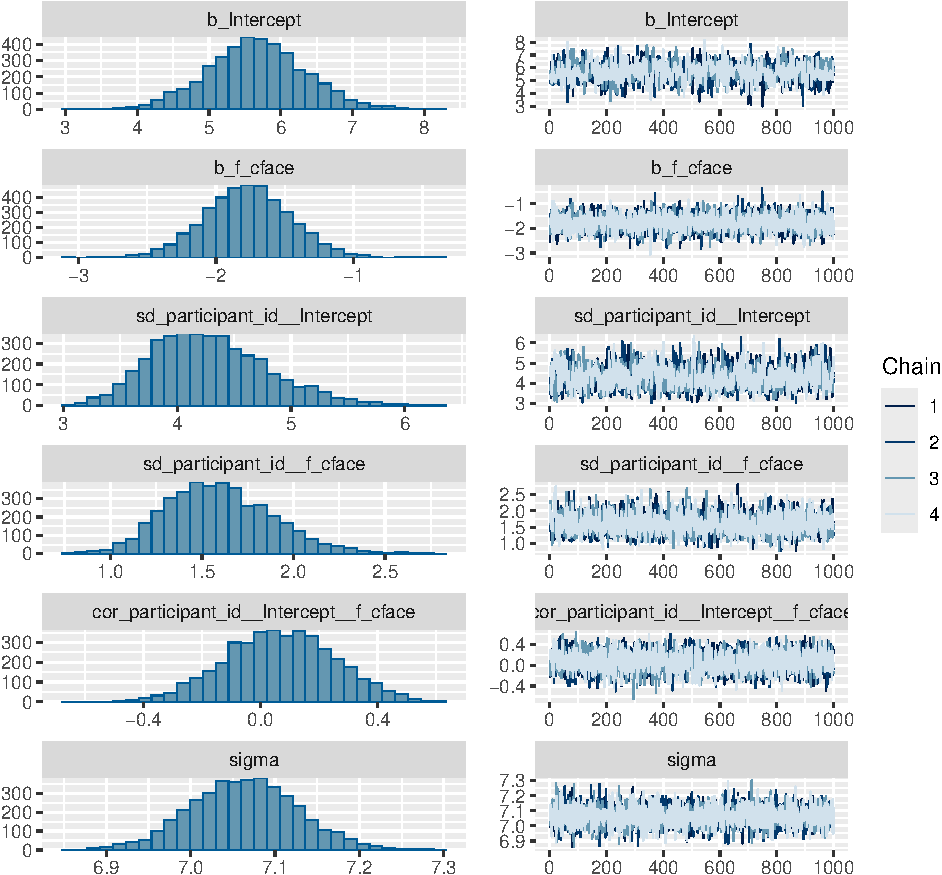
\includegraphics{bachelor_thesis_files/figure-latex/plot-blmm-1.pdf}
\caption{\label{fig:plot-blmm}Posterior distributions and trace plots of the correlation model}
\end{figure}

So far, we have looked at the specification and the results of the BLMM without specifying the concrete prior distributions. In the next section, we will look at how to set these priors appropriately.

\subsection{Prior Elicitation}\label{prior-elicitation}

Probably the most frequently asked question about Bayesian statistics is how to determine the priors. For researchers with a frequentist background this often seems like a daunting task with a lot of subjectivity. However, while it does increase the researchers degrees of freedom and remains a difficult task even for expert statisticians, there are some paths you can follow to find appropriate priors. As we have seen in Section 2.3, prior distributions encode the a priori knowledge about the parameters. Ideally prior distributions should therefore be elicited without any knowledge of the collected data, incorporating only the information available prior to the measurement (Gelman et al., 2017). In the prior elicitation we are trying to translate the already available domain knowledge into probability distributions (Mikkola et al., 2023). There are different approaches to it and the priors we choose can have different characteristics, depending on the approach.

In the following analysis we will be using so called principled priors (Nicenboim et al., n.d., para. 3.4). Principled priors encode all the theory-neutral information. In our case that means all the information about ERPs and EEG data in general, but not for example the direction of the N170 effect. To acquire this domain knowledge typically a mix of several sources of information is used, one's own experience, previous experiments, meta-analyses, expert knowledge, anything that can be ruled out by logic or invariances (Lee \& Vanpaemel, 2018; Nicenboim et al., n.d.). To reduce the influence of biases on the final results, the analyses are typically carried out with more than one prior.

Looking back to Eq. \eqref{eq:BLMM} and \eqref{eq:priors-BLMM} we can see that we need priors for six different parameters, the fixed intercept \(\beta_0\), the fixed slope \(\beta_1\), the variance component of the random intercept and random slope \(\tau_0\) and \(\tau_1\), the within subject variance component \(\sigma\) and the correlation between random intercept and random slope \(\rho_u\). For each parameter we will briefly look at what we already know about this parameter and how this can be translated into a probability distribution. In the present tutorial, the elicitation process is kept short, only to demonstrate the concept. In an actual analysis this is a very important step before analyzing the data and should be done thoroughly.

For the fixed intercept we will take most of our information from the preprocessing steps. During preprocessing, the data were rereferenced to average, for each epoch, the average voltage of the entire time window was then subtracted from all time points of the epoch at every channel and epochs were rejected when the peak-to-peak amplitude exceeded 200 \(\mu\)V. Finally, every single data point of the analysis is the average at the region of interest over a specific time window. All of these processing steps result in the single trial average being shifted closer to zero. So, independent of what ERP component we are looking at, we will expect the mean amplitude to be some \(\mu V\) around zero. Additionally, looking at mean amplitudes from different ERP effects and more specifically the N170, almost all of them are smaller than 10 \(\mu V\) (e.g. Kappenman et al., 2021; Nan et al., 2022). This is why we will be using a prior of \(N(0, 10)\), placing the bulk of the distribution between -10 and 10 \(\mu V\) while at the same time allowing for a wider range if necessary.

The fixed slope represents our main experimental effect, the difference in the N170 between seeing faces and seeing cars. In general, ERP effects are only a few of \(\mu V\) large (e.g. Enge et al., 2023; Frömer et al., 2018; Kappenman et al., 2021) even with large effects like the N400 (Nieuwland et al., 2018). As this also holds for the N170 (e.g. Itier \& Taylor, 2004) we will set the prior to \(N(0, 10)\). This places the bulk of the distribution between -10 and 10 \(\mu V\), which represents our expectations, while still allowing for slopes outside that range.

As EEG random intercepts and slopes are only rarely reported, we had little information to go by. Based on the study from Frömer et al. (2018), we could infer the standard deviation of the random effects are rather small, but this could of course be unique to their study. Therefore we will be using a wider prior to allow for other possibilities. As the standard deviation is always positive, we will use a truncated normal distribution of \(N_+(0, 20)\).

The \(\sigma\) represents the within person variance, which is assumed to be the same for all participants. As we cannot rely on previous Bayesian analysis of EEG data we do not have any information on how the prior for sigma should look like. We only know that \(\sigma\) has to be greater than zero as it is a standard deviation. We will also assume within person variance to be greater than between person variance because the latter is reduced through averaging within a participant. We again use a truncated normal distribution \(N_+(0, 50)\) with a higher standard deviation compared to the random effects. This leaves us with a very wide prior, which accurately reflects how little knowledge we have.

For the correlation between random intercept and slope we are using an LKJ distribution (Joe, 2006; Lewandowski et al., 2009). Because the correlation is seldom reported, we have little knowledge on what to expect it to be for our data. This is why we chose a rather uninformative prior. With a prior of \(LKJ(2)\) we express a slight preference for small correlations while the entire range of correlations (from -1 to 1) is still possible. This leaves room for different correlations and does not bias the analysis.

All of these considerations leave us with the following priors.

\begin{Shaded}
\begin{Highlighting}[]
\CommentTok{\# Setting the prior}
\NormalTok{prior\_1 }\OtherTok{\textless{}{-}} \FunctionTok{c}\NormalTok{(}
  \CommentTok{\# fixed Intercept}
  \FunctionTok{prior}\NormalTok{(}\FunctionTok{normal}\NormalTok{(}\DecValTok{0}\NormalTok{, }\DecValTok{10}\NormalTok{), }\AttributeTok{class =}\NormalTok{ Intercept), }
  \CommentTok{\# fixed slope}
  \FunctionTok{prior}\NormalTok{(}\FunctionTok{normal}\NormalTok{(}\DecValTok{0}\NormalTok{, }\DecValTok{10}\NormalTok{), }\AttributeTok{class =}\NormalTok{ b, }\AttributeTok{coef =}\NormalTok{ f\_cface), }
  \CommentTok{\# within person variation}
  \FunctionTok{prior}\NormalTok{(}\FunctionTok{normal}\NormalTok{(}\DecValTok{0}\NormalTok{, }\DecValTok{50}\NormalTok{), }\AttributeTok{class =}\NormalTok{ sigma), }
  \CommentTok{\# between person variation in mean}
  \FunctionTok{prior}\NormalTok{(}\FunctionTok{normal}\NormalTok{(}\DecValTok{0}\NormalTok{, }\DecValTok{20}\NormalTok{), }\AttributeTok{class =}\NormalTok{ sd, }\AttributeTok{coef =}\NormalTok{ Intercept, }
        \AttributeTok{group =}\NormalTok{ participant\_id), }
  \CommentTok{\# between person variation in slope}
  \FunctionTok{prior}\NormalTok{(}\FunctionTok{normal}\NormalTok{(}\DecValTok{0}\NormalTok{, }\DecValTok{20}\NormalTok{), }\AttributeTok{class =}\NormalTok{ sd, }\AttributeTok{coef =}\NormalTok{ f\_cface, }
        \AttributeTok{group =}\NormalTok{ participant\_id), }
  \CommentTok{\# correlation between random intercept and slope}
  \FunctionTok{prior}\NormalTok{(}\FunctionTok{lkj}\NormalTok{(}\DecValTok{2}\NormalTok{), }\AttributeTok{class =}\NormalTok{ cor, }\AttributeTok{group =}\NormalTok{ participant\_id)}
\NormalTok{) }
\end{Highlighting}
\end{Shaded}

\subsection{Prior Predictive Checks}\label{prior-predictive-checks}

After deciding on a prior distribution for each parameter, it is important to confirm that the priors are appropriate, indeed. One essential way to check the plausibility of the priors is to do prior predictive checks. This is a form of sensitivity analysis to investigate possible biases of the prior and to assess whether it may be too vague. The prior predictive checks compute a posterior distribution by using only the prior and not the likelihood. This allows us to evaluate whether the prior covers all the possible outcomes of our experiment. Typically, it should be a bit wider than the outcomes we would expect, to rule out any biases. These checks are typically performed for several different priors to compare them.

Prior predictive checks can easily be performed in R by setting the \texttt{sample\_prior} argument in the \texttt{brm} function to \texttt{"only"}.

\begin{Shaded}
\begin{Highlighting}[]
\CommentTok{\# Fitting the BLMM for a prior predictive check}
\NormalTok{mod\_ppc }\OtherTok{\textless{}{-}} \FunctionTok{brm}\NormalTok{(N170 }\SpecialCharTok{\textasciitilde{}} \DecValTok{1} \SpecialCharTok{+}\NormalTok{ f\_c }\SpecialCharTok{+}\NormalTok{ (}\DecValTok{1} \SpecialCharTok{+}\NormalTok{ f\_c }\SpecialCharTok{|}\NormalTok{ participant\_id),}
               \AttributeTok{data =}\NormalTok{ trials\_cond, }
               \AttributeTok{prior =}\NormalTok{ prior\_1,}
               \AttributeTok{family =} \FunctionTok{gaussian}\NormalTok{(),}
               \AttributeTok{sample\_prior =} \StringTok{"only"}\NormalTok{, }\CommentTok{\# use only the prior distribution}
               \AttributeTok{cores =} \DecValTok{4}\NormalTok{) }
\end{Highlighting}
\end{Shaded}

For each parameter we can now examine the posterior distribution (Fig. \ref{fig:prior-model-plot}). These distributions visualize the priors we set in Section 2.4, because the actual data were not included in the model. As in the prior elicitation process, we again want to check whether these distributions reflect our domain knowledge. For each posterior, we can ask ourselves whether an actual data set could be found in the distribution. For example, looking at the main fixed effect \(b_1\) (called \texttt{b\_f\_cface}), the bulk of the distribution is between -10 and 10 and this matches our knowledge that most ERP effects are only a couple of \(\mu V\) small (e.g. Enge et al., 2023; Frömer et al., 2018; Kappenman et al., 2021). To rule out any bias however, we want our prior to be a bit wider than what we would expect. That way, even if our knowledge is not completely accurate, almost all experiments would still fall into the range of our prior. As the range of the \(b_1\) prior is indeed wider than -10 to 10 \(\mu V\) (approximately -20 to 20 \(\mu V\)) this requirement is also fulfilled with our choice of prior.



\begin{figure}
\centering
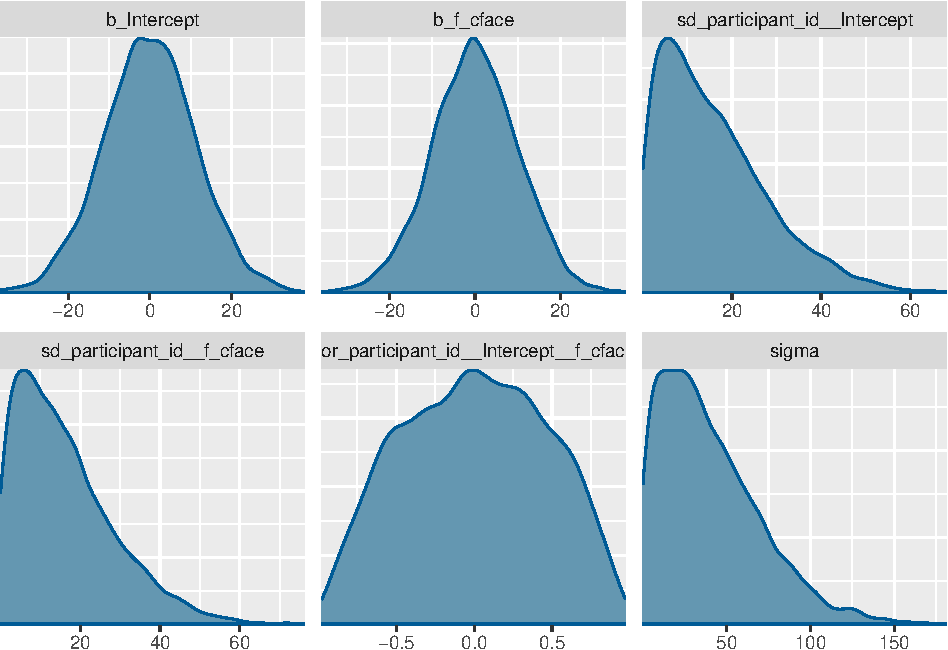
\includegraphics{bachelor_thesis_files/figure-latex/prior-model-plot-1.pdf}
\caption{\label{fig:prior-model-plot}Posterior distributions of the parameters of the prior predictive model}
\end{figure}

It can be difficult, however, to picture how an actual data set with these priors would look like. This is why we additionally look at samples drawn from the prior predictive model. These samples represent how the model predicts possible data sets to look like. With the \texttt{pp\_check} function, we can visualize histograms of these samples. The \texttt{prefix} ``ppd'' specifies that we are performing prior predictive checks and do not want the original data set to be shown alongside the sample data sets. Already comparing the samples with our actual data might bias us in a certain direction. As we have seen in Section 2.4, we would assume our data set to be approximately normally distributed around zero, not exceeding -100 \(\mu V\) and 100 \(\mu V\). For the standard distribution we used a very vague prior, so we would assume some variance here. And this is what we actually see in Fig. \ref{fig:prior-predictive}. The bounds of our samples sometimes exceed the \(+/-\) 100 \(\mu V\) we expect, but, as we usually want our priors to be a bit wider than our assumptions, this does not pose a problem. The standard deviation of our posterior samples varies substantially as expected. Unfortunately, the lack of previous EEG experiments using Bayesian methods makes it difficult to determine a good prior for \(\sigma\). In such a case, using a wider prior is usually the preferred option to not introduce any bias. In summary, our predictive samples seem to match our expectations after prior elicitation.



\begin{Shaded}
\begin{Highlighting}[]
\FunctionTok{pp\_check}\NormalTok{(mod\_ppc, }\AttributeTok{ndraws =} \DecValTok{12}\NormalTok{, }\AttributeTok{type =} \StringTok{"hist"}\NormalTok{, }\AttributeTok{prefix =} \FunctionTok{c}\NormalTok{(}\StringTok{"ppd"}\NormalTok{))}
\end{Highlighting}
\end{Shaded}

\begin{figure}
\centering
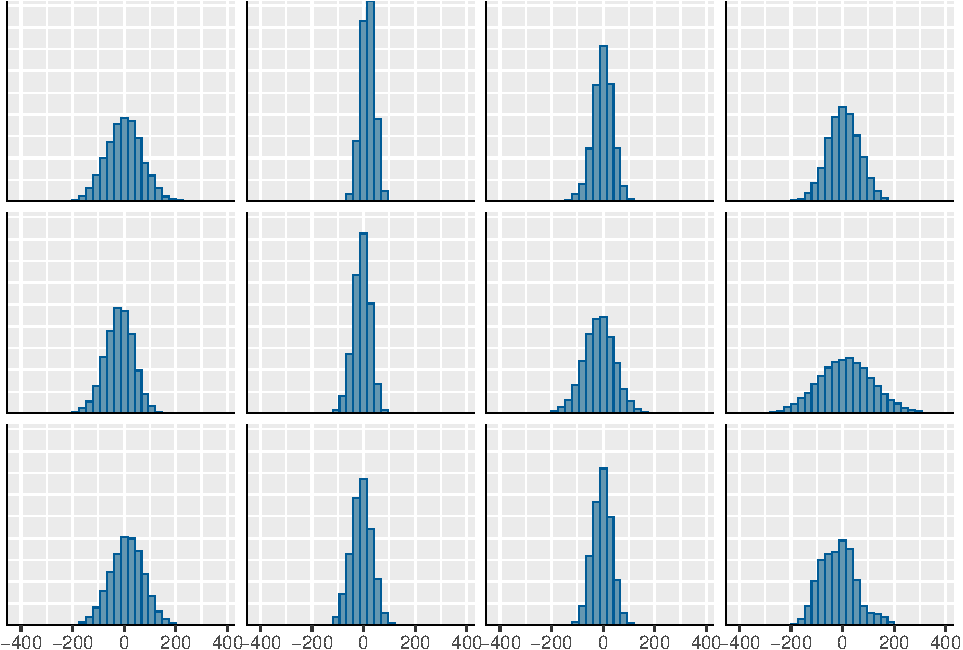
\includegraphics{bachelor_thesis_files/figure-latex/prior-predictive-1.pdf}
\caption{\label{fig:prior-predictive}Sample data sets drawn from the prior predictive model}
\end{figure}

\subsection{Sampling and Convergence}\label{sampling-and-convergence}

For the estimation of the model parameters we need to work out the posterior distribution of our model. In most cases, however, the marginal likelihood cannot be computed analytically. Therefore, we have to rely on sampling to compute the posterior distribution. With enough samples, we will get a good approximation of the posterior. When performing the analysis of Bayesian models with Stan (Stan Development Team, 2024) or an interface of it, like brms (Bürkner, 2018), the sampling is done using an algorithm called Markov Chain Monte Carlo or, more specifically, Hamiltonian Monte Carlo (HMC, Carpenter et al., 2017; for a conceptual introduction to MCMC algorithms see Betancourt, 2018). HMC draws sample data sets out of the high dimensional parameter space created by the prior and the likelihood in a way that reflects the posterior distribution. These samples then act as a simulation of the posterior and allow us to extract the distributions of the parameters important to us. This process is usually done several times in different so called chains. The brms package uses four chains per default which follows the recommendation by Vehtari et al. (2021). Each chain undergoes the sampling process independently and the results are then combined. Because the starting point of each chain is picked randomly and the algorithm might need some iterations to get to the region of interest, the first iterations are usually treated as a warm-up phase and discarded afterwards. The remaining samples are then forming the new posterior distribution. The default number of iterations in brms is usually a good start, but we will also see situations in which more iterations are necessary.

In infinite time, this algorithm would always lead to the correct posterior distribution (Roy, 2020). But of course we only have limited time resources. That is why we need to check whether the algorithm converged properly in the amount of iterations we set. We can do so by looking at some convergence criteria. The most commonly used convergence diagnostics are \(\hat{R}\) and the effective sample sizes (Vehtari et al., 2021). Roughly speaking, the \(\hat{R}\) compares the between- and within-chain variance. If the variance of all the chains put together is greater than the variance of one single chain, we conlcude the sampling has not worked properly. Ideally, every \(\hat{R}\) should be 1, but a good threshold seems for \(\hat{R}\) to not be greater than 1.01 (Vehtari et al., 2021). The effective sample size (ESS) reflects the number of independent samples that would contain the same amount of information as the set of correlated samples we get after running the MCMC algorithm (Roy, 2020). We aim for as many effective samples as possible, but at least 400 for every parameter (Vehtari et al., 2021).

The summary of the \texttt{brm}-model gives us some information on the convergence of our model. If the model did not converge properly we also get a warning from Stan. The estimated \(\hat{R}\) can be found under \texttt{Rhat} and the effective sample sizes under \texttt{Bulk\_ESS} for the major part of the posterior distribution and \texttt{Tail\_ESS} for the tails. As we can see in the output of the model from Section 2.3, it converged nicely. All the \(\hat{R}\)s are smaller or equal to 1 and we have an ESS of at least 737 for every parameter. The trace plot (see Fig. \ref{fig:plot-blmm}) of the model also look like we would expect, hovering equally around the mean of each distribution.

If the sampling did not work properly there are several options to address this (see Gelman (n.d.)). First, we should check whether the model is properly defined. Then, we can either use more informative (smaller) priors to constrain the sampling space or increase the number of iterations. Having said that, small deviations from the recommendations (e.g., if the \texttt{Tail\_ESS} is only 370 for one parameter) are usually not a problem and the model fit should always be looked at as a whole.

\subsection{Posterior Predictive Checks}\label{posterior-predictive-checks}

After computing the complete model and confirming that it converged properly, we can take look at the posterior distribution to determine its descriptive adequacy (Shiffrin et al., 2008). We want to determine whether the data predicted by the model are reasonable. This is usually done via posterior predictive checks. In Section 2.5 we have seen that we can draw samples from the posterior distribution of the model. We now want to assess the model's ability to predict data sets similar to our own. Although this cannot be seen as good evidence for the model, an inadequacy in properly predicting similar data sets strongly speaks against the model (Shiffrin et al., 2008). Posterior predictive checks can give a first impression of the model predictions, but it should only be seen as a sanity check (Nicenboim et al., n.d.). For model comparison, different criteria should be used to assess the performance of a model {[}e.g. Roberts and Pashler (2000); xxx{]}. As for the prior predictive checks, posterior predictive checks should be done for a few different priors, to assess the influence of the prior on the posterior distribution.

To perform posterior predictive checks, we can again use the \texttt{pp\_check} function. Looking at Fig \ref{fig:posterior-check-blmm-hist}, the samples indeed look very similar to our observed data. The only difference seems to be a slightly smaller standard deviation, the actual data set has a higher peak and a narrower distribution. Apart from that, the model predicts data sets closely related to the observed data. For EEG experiments, this will usually be the case, because we have so many data points and the prior plays a smaller role in the posterior predictive distribution.



\begin{Shaded}
\begin{Highlighting}[]
\FunctionTok{pp\_check}\NormalTok{(mod\_blmm, }\AttributeTok{ndraws =} \DecValTok{11}\NormalTok{, }\AttributeTok{type =} \StringTok{"hist"}\NormalTok{)}
\end{Highlighting}
\end{Shaded}

\begin{figure}
\centering
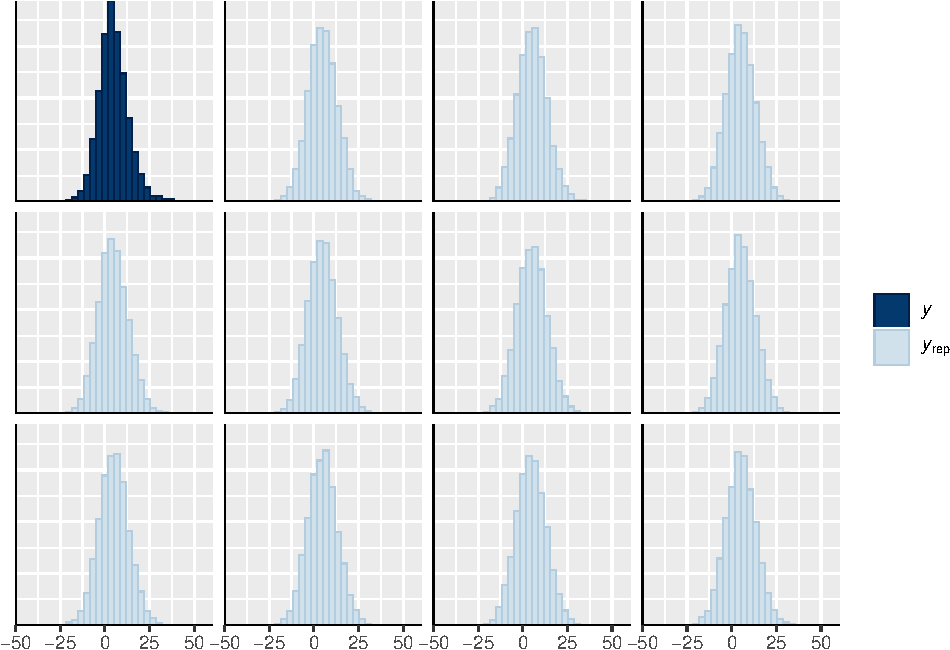
\includegraphics{bachelor_thesis_files/figure-latex/posterior-check-blmm-hist-1.pdf}
\caption{\label{fig:posterior-check-blmm-hist}Histograms of the original data set and of samples drawn from the posterior predictive distribution}
\end{figure}

When specifying the \texttt{type} of the \texttt{pp\_check} function as \texttt{"dens-overlay"}, we can directly compare the distributions of our predicted samples with the actual data set (see Fig. \ref{fig:posterior-check-blmm-density}). This emphasizes the small difference between the actual data and the predicted samples. The model does not cover all the information contained in the data. In the next section we will introduce a new model to account for this difference.



\begin{Shaded}
\begin{Highlighting}[]
\FunctionTok{pp\_check}\NormalTok{(mod\_blmm, }\AttributeTok{ndraws =} \DecValTok{100}\NormalTok{, }\AttributeTok{type =} \StringTok{"dens\_overlay"}\NormalTok{)}
\end{Highlighting}
\end{Shaded}

\begin{figure}
\centering
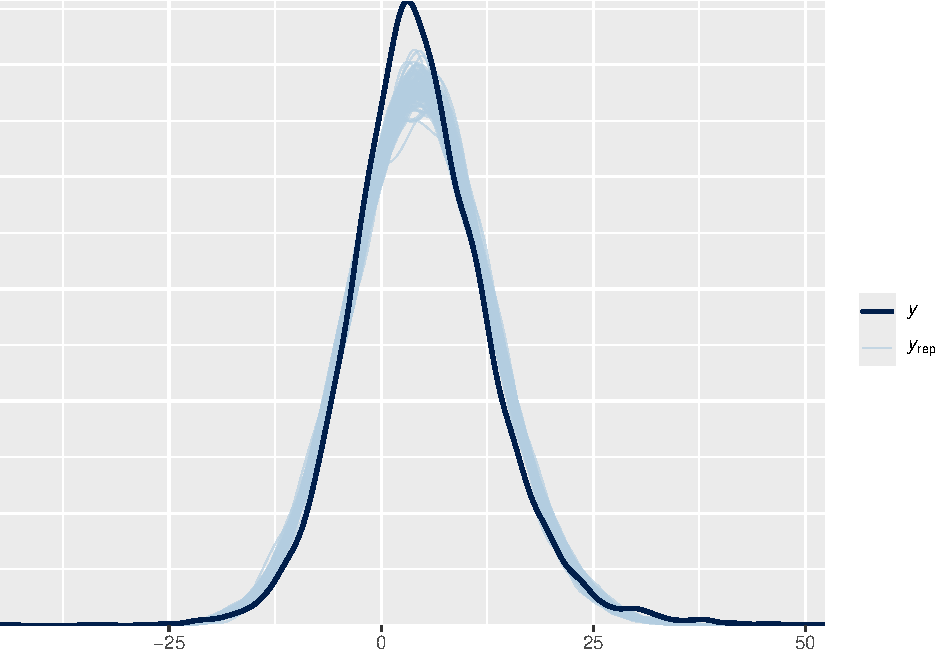
\includegraphics{bachelor_thesis_files/figure-latex/posterior-check-blmm-density-1.pdf}
\caption{\label{fig:posterior-check-blmm-density}Density plot of the original data set and of samples drawn from the posterior predictive distribution}
\end{figure}

\subsection{Distributional Regression}\label{distributional-regression}

As we have seen in the previous section, there is a part of the signal distribution that the model cannot account for. This could be explained by a high variance of noise levels between participants (Nicenboim et al., n.d.). In ERP studies, the level of impedance between skin and electrodes has a significant effect on the amount of noise in the data (Picton et al., 2000). Since the impedance is depending on the skin tissue of each participant, the amount of noise might vary a lot. We can check this hypothesis with the following code that shows posterior samples grouped by participant.



\begin{Shaded}
\begin{Highlighting}[]
\CommentTok{\# Posterior predictive check by participant}
\FunctionTok{pp\_check}\NormalTok{(mod\_blmm, }
         \AttributeTok{type =} \StringTok{"dens\_overlay\_grouped"}\NormalTok{,}
         \AttributeTok{ndraws =} \DecValTok{100}\NormalTok{,}
         \AttributeTok{group =} \StringTok{"participant\_id"}\NormalTok{)}
\end{Highlighting}
\end{Shaded}

\begin{figure}
\centering
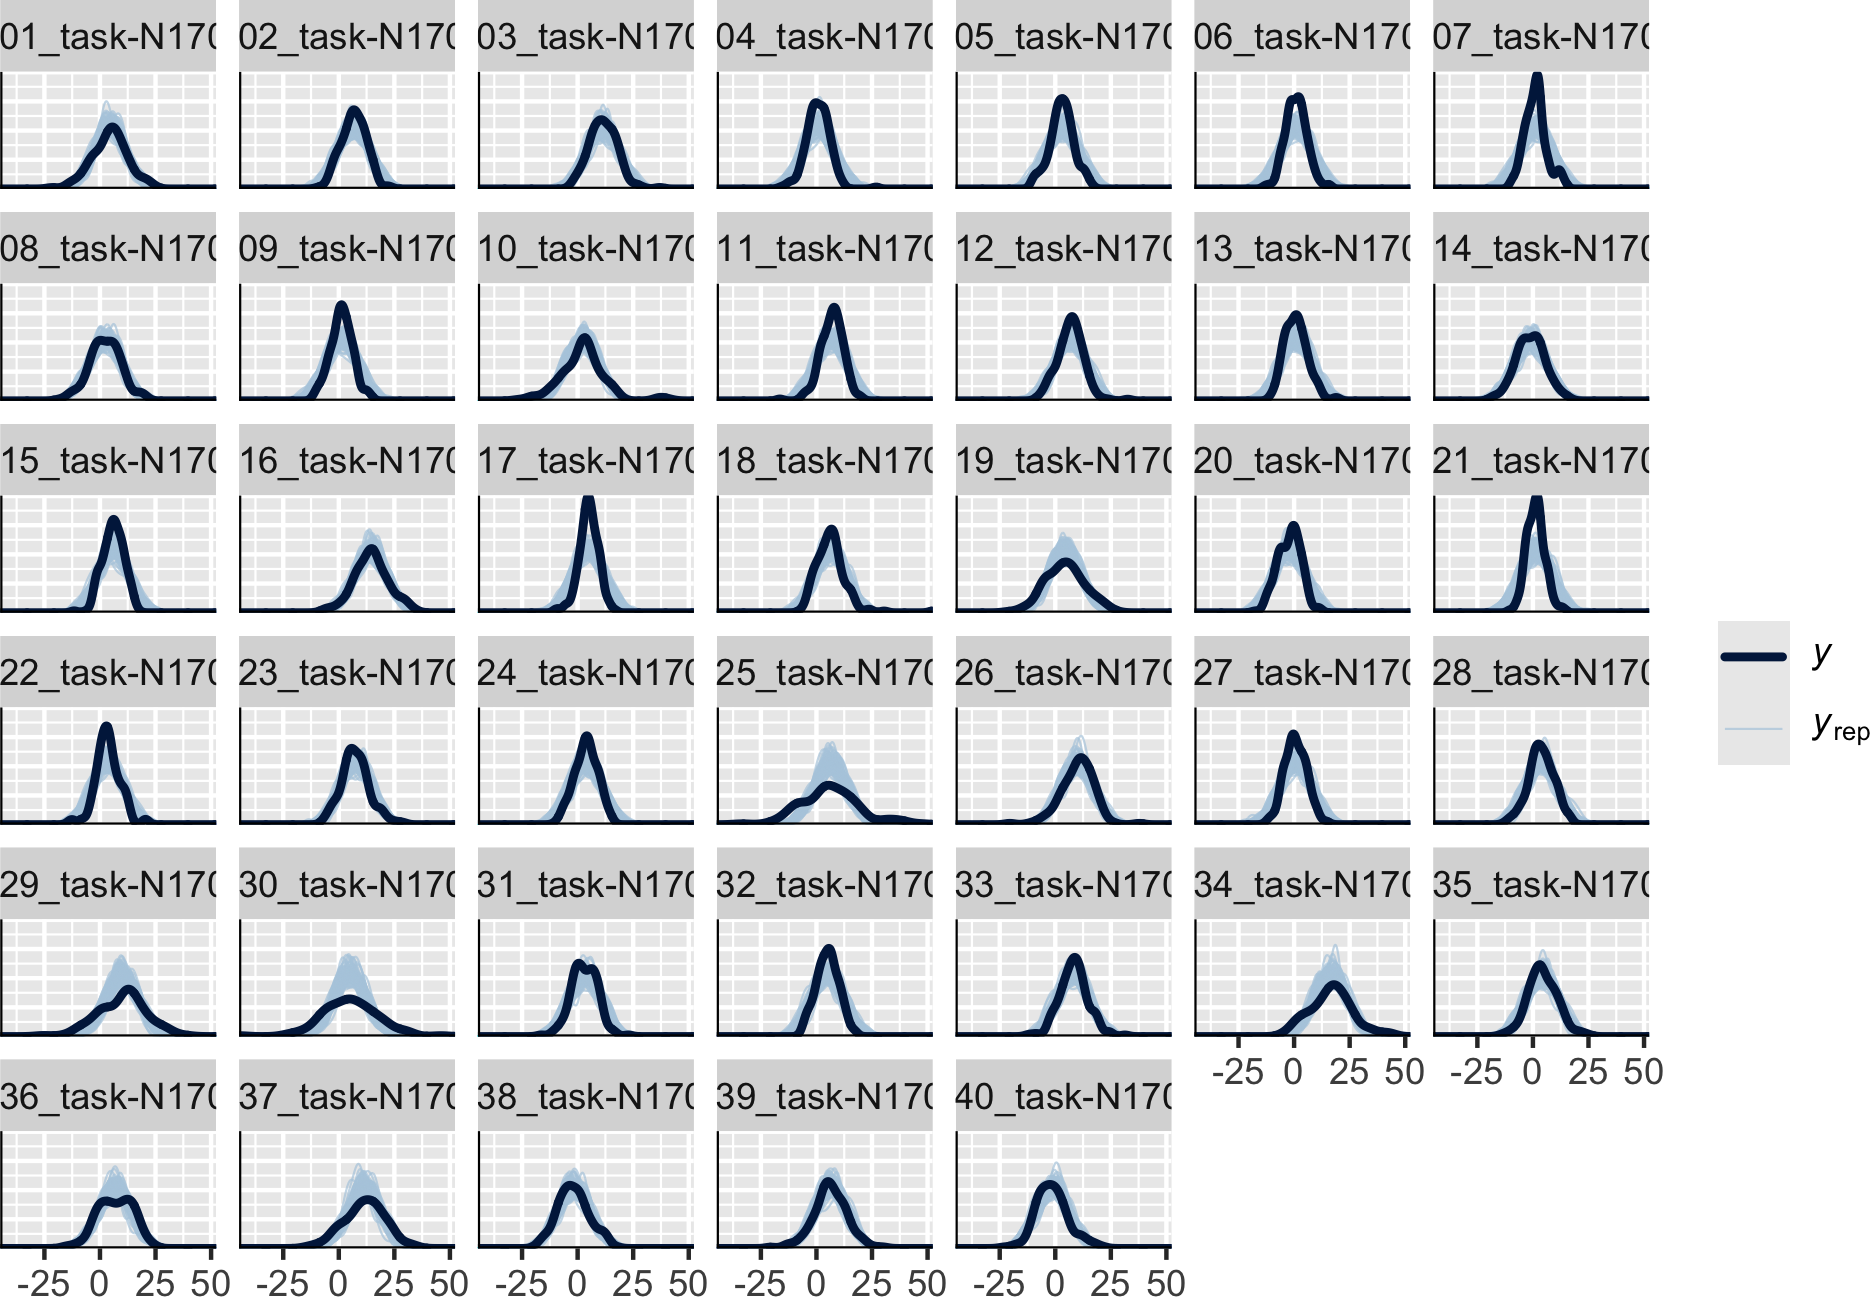
\includegraphics{bachelor_thesis_files/figure-latex/sigma-variance-1.pdf}
\caption{\label{fig:sigma-variance}Predicted distributions of the N170 signal data grouped by participant}
\end{figure}



\begin{Shaded}
\begin{Highlighting}[]
\FunctionTok{pp\_check}\NormalTok{(mod\_blmm,}
         \AttributeTok{type =} \StringTok{"stat\_grouped"}\NormalTok{,}
         \AttributeTok{ndraws =} \DecValTok{1000}\NormalTok{,}
         \AttributeTok{group =} \StringTok{"participant\_id"}\NormalTok{,}
         \AttributeTok{stat =} \StringTok{"sd"}\NormalTok{,}
         \AttributeTok{facet\_args =} \FunctionTok{list}\NormalTok{(}\AttributeTok{scales =} \StringTok{"fixed"}\NormalTok{))}
\end{Highlighting}
\end{Shaded}

\begin{figure}
\centering
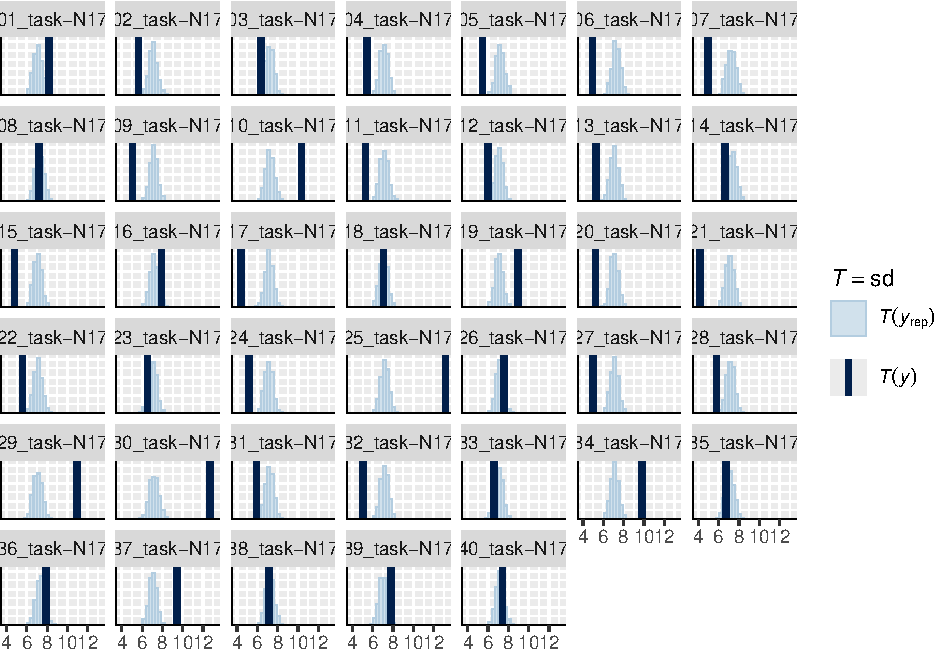
\includegraphics{bachelor_thesis_files/figure-latex/sigma-variance-sd-1.pdf}
\caption{\label{fig:sigma-variance-sd}Predicted standard deviations of the N170 signal data grouped by participant}
\end{figure}

As we can see in Fig. \ref{fig:sigma-variance} and \ref{fig:sigma-variance-sd} there are indeed highly varying noise levels between the participants that our current model does not capture. By assuming the same within-person variance \(\sigma\) for all participants we might be misfitting participants with significantly lower or higher \(\sigma\) (Nicenboim et al., n.d.). To account for these differences we will look at a new kind of statistical model.

Models in psychology usually look at mean differences. Whether we look at differences between groups, experimental conditions or individuals, difference is commonly defined as difference in mean. Differences in scale or shape are just regarded a nuisance because they might violate the assumptions of our models (e.g., the homoscedasticity assumption in linear models). In distributional models, also called generalized additive models for location, scale and shape (GAMLSS), the entire distribution is modeled for each group or individual separately, therefore incorporating any differences in scale or shape into the model (Klein, 2024). With these models, differences in noise levels could be modeled instead of being ignored. Fortunately, the brms package allows for an easy extension to distributional regression (Bürkner, 2018, 2024). This emphasizes the flexibility of the Bayesian framework, enabling us to conveniently adapt to the data at hand. The computational back-end using modern MCMC algorithms is also powerful enough to estimate these much more complex models (Bürkner, 2024; see Kneib et al., 2023 for a review of distributional regression approaches).

\subsubsection{Mathematical Model and Implementation in R}\label{mathematical-model-and-implementation-in-r-1}

In our case, we assume that the shape of the signal remains a normal distribution for every participant, only the variance of this normal distribution can differ between participants. We thereby introduce the hierarchical structure of our data also into the variance component.

The formal model will change in a way that the single trial averages will now have a person-specific \(\sigma\). The \(\sigma\) is hence dependent on which person the trial belongs to but does not differ for the experimental condition. We do not expect the condition of faces vs.~cars to influence the signal variance. We exponentiate \(\sigma\) so that it cannot become negative even with negative adjustments (Nicenboim et al., n.d.). Equation \eqref{eq:dist-reg} shows our new model.

\begin{equation}
\begin{split}
& y_{ij} \sim N(\beta_0 + u_{j,1} + X_{ij}(\beta_1 + u_{j,2}), \enspace \sigma_j) \\
& With \enspace \sigma_j = exp(\sigma_{\beta_0} + \sigma_{u_j})
\end{split}
\label{eq:dist-reg}
\end{equation}

We also need to add priors to the new parameters. Since no ERP studies have used distributional models so far we, have very little prior knowledge on how the parameters behave. Therefore, we first remained with the previous prior for the intercept of the sigma (now as log(50) because it will be exponentiated afterwards). For the variance component of sigma we chose a rather uninformative prior.

\begin{equation}
\begin{split}
& \sigma_{\beta_0} \sim N(0, log(50)) \\
& \sigma_{u_j} \sim N(0, \tau_{\sigma_u}) \\
& \tau_{\sigma_u} \sim N_{+}(0,5)
\end{split}
\label{eq:prior-dist}
\end{equation}

By performing a sensitivity analysis using prior predictive checks we have then verified whether our chosen priors were actually sensible. This allowed us to see that the priors in Eq. \eqref{eq:prior-dist} are too broad and the means of the signal averages are too spread out. We will not look at the prior predictive checks in detail here, because the concept remains the same, further details can be found in the corresponding script. Following the sensitivity analysis, we have then decided on the following prior, denoted by \texttt{dpar\ =\ sigma} (distributional parameter).

\begin{Shaded}
\begin{Highlighting}[]
\CommentTok{\# Prior for distributional regression}
\NormalTok{prior\_dist }\OtherTok{\textless{}{-}} \FunctionTok{c}\NormalTok{(}
  \FunctionTok{prior}\NormalTok{(}\FunctionTok{normal}\NormalTok{(}\DecValTok{0}\NormalTok{, }\DecValTok{10}\NormalTok{), }\AttributeTok{class =}\NormalTok{ Intercept), }
  \FunctionTok{prior}\NormalTok{(}\FunctionTok{normal}\NormalTok{(}\DecValTok{0}\NormalTok{, }\DecValTok{10}\NormalTok{), }\AttributeTok{class =}\NormalTok{ b, }\AttributeTok{coef =}\NormalTok{ f\_cface),}
  \CommentTok{\# intercept of sigma}
  \FunctionTok{prior}\NormalTok{(}\FunctionTok{normal}\NormalTok{(}\DecValTok{0}\NormalTok{, }\FunctionTok{log}\NormalTok{(}\DecValTok{3}\NormalTok{)), }\AttributeTok{class =}\NormalTok{ Intercept, }\AttributeTok{dpar =}\NormalTok{ sigma), }
  \CommentTok{\# variance component of sigma}
  \FunctionTok{prior}\NormalTok{(}\FunctionTok{normal}\NormalTok{(}\DecValTok{0}\NormalTok{, }\DecValTok{1}\NormalTok{), }\AttributeTok{class =}\NormalTok{ sd, }
        \AttributeTok{group =}\NormalTok{ participant\_id, }\AttributeTok{dpar =}\NormalTok{ sigma), }
  \FunctionTok{prior}\NormalTok{(}\FunctionTok{normal}\NormalTok{(}\DecValTok{0}\NormalTok{, }\DecValTok{20}\NormalTok{), }\AttributeTok{class =}\NormalTok{ sd, }\AttributeTok{coef =}\NormalTok{ Intercept, }
        \AttributeTok{group =}\NormalTok{ participant\_id),  }
  \FunctionTok{prior}\NormalTok{(}\FunctionTok{normal}\NormalTok{(}\DecValTok{0}\NormalTok{, }\DecValTok{20}\NormalTok{), }\AttributeTok{class =}\NormalTok{ sd, }\AttributeTok{coef =}\NormalTok{ f\_cface, }
        \AttributeTok{group =}\NormalTok{ participant\_id), }
  \FunctionTok{prior}\NormalTok{(}\FunctionTok{lkj}\NormalTok{(}\DecValTok{2}\NormalTok{), }\AttributeTok{class =}\NormalTok{ cor, }\AttributeTok{group =}\NormalTok{ participant\_id)}
\NormalTok{  ) }
\end{Highlighting}
\end{Shaded}

To fit our model in brms, we need to use the function \texttt{brmsformula} (or its alias \texttt{bf}) (Bürkner, 2024). This function allows to extend the current formula to a distributional regression, applying the hierarchical nature of the data to any parameter. The first part inside the \texttt{bf} function stays the same, the second part, after the comma, allows us to specify the structure of the distributional part. As mentioned before, in our case the scale (sigma) of the distribution will only depend on the participant, we are therefore adding a random effect here. We fit the model with increased iterations (\texttt{iter}) due to the higher complexity of the model (a new parameter must be fitted for each participant).

\begin{Shaded}
\begin{Highlighting}[]
\CommentTok{\# Distributional regression model }
\NormalTok{mod\_dist }\OtherTok{\textless{}{-}} \FunctionTok{brm}\NormalTok{(}\FunctionTok{bf}\NormalTok{(N170 }\SpecialCharTok{\textasciitilde{}} \DecValTok{1} \SpecialCharTok{+}\NormalTok{ f\_c }\SpecialCharTok{+}\NormalTok{ (}\DecValTok{1} \SpecialCharTok{+}\NormalTok{ f\_c }\SpecialCharTok{|}\NormalTok{ participant\_id), }
\NormalTok{                   sigma }\SpecialCharTok{\textasciitilde{}} \DecValTok{1} \SpecialCharTok{+}\NormalTok{ (}\DecValTok{1} \SpecialCharTok{|}\NormalTok{ participant\_id)), }
                \AttributeTok{data =}\NormalTok{ trials\_cond, }
                \AttributeTok{prior =}\NormalTok{ prior\_dist,}
                \AttributeTok{family =} \FunctionTok{gaussian}\NormalTok{(),}
                \AttributeTok{iter =} \DecValTok{4000}\NormalTok{,}
                \AttributeTok{warmup =} \DecValTok{1000}\NormalTok{,}
                \AttributeTok{cores =} \DecValTok{4}\NormalTok{) }
\end{Highlighting}
\end{Shaded}

\subsubsection{Results}\label{results-2}

As before, we will first take a look at the output of the \texttt{summary} function to get an overview of our fitted model.



\footnotesize

\begin{verbatim}
##  Family: gaussian 
##   Links: mu = identity; sigma = log 
## Formula: N170 ~ 1 + f_c + (1 + f_c | participant_id) 
##          sigma ~ 1 + (1 | participant_id)
##    Data: trials_cond (Number of observations: 6224) 
##   Draws: 4 chains, each with iter = 4000; warmup = 1000; thin = 1;
##          total post-warmup draws = 12000
## 
## Multilevel Hyperparameters:
## ~participant_id (Number of levels: 40) 
##                        Estimate Est.Error l-95% CI u-95% CI Rhat Bulk_ESS
## sd(Intercept)              4.32      0.54     3.41     5.50 1.00     1945
## sd(f_cface)                1.55      0.28     1.06     2.16 1.00     4195
## sd(sigma_Intercept)        0.30      0.04     0.24     0.38 1.00     1880
## cor(Intercept,f_cface)     0.06      0.19    -0.31     0.43 1.00     4889
##                        Tail_ESS
## sd(Intercept)              3863
## sd(f_cface)                6961
## sd(sigma_Intercept)        4359
## cor(Intercept,f_cface)     7328
## 
## Regression Coefficients:
##                 Estimate Est.Error l-95% CI u-95% CI Rhat Bulk_ESS Tail_ESS
## Intercept           5.63      0.70     4.25     7.01 1.01      845     2003
## sigma_Intercept     1.87      0.05     1.77     1.96 1.00     1286     2267
## f_cface            -1.76      0.30    -2.34    -1.15 1.00     4064     6491
## 
## Draws were sampled using sampling(NUTS). For each parameter, Bulk_ESS
## and Tail_ESS are effective sample size measures, and Rhat is the potential
## scale reduction factor on split chains (at convergence, Rhat = 1).
\end{verbatim}

\normalsize

Notice that the estimate of the main effect, the difference between the perception of faces and cars in the N170, remains almost the same with \(b_1\) = -1.76 compared to \(b_1\) = -1.77 in the standard BLMM. The same holds for the intercept which also changes only slightly to \(b_0\) = 5.63 (compared to \(b_0\) = 5.66). The two new parameters in our distributional model are referred to as \texttt{sigma\_Intercept} for the intercept of the sigma and \texttt{sd(sigma\_intercept)} for the variance component of sigma. The model also seems to have converged nicely, as all \(\hat{R}\)s are under \(1.01\) and the ESS are at a minimum of 845.

Despite the small differences in the point estimates, by performing a posterior predictive check it becomes clear that the new model can fit our data better than the old one (see Fig. \ref{fig:posterior-check-dist}), fitting every part of the distribution. Accounting for the differences in noise level between participants seems to have made a difference for the model fit, at least on a visual level. This leads us to expect an improved prediction capacity of the model. In the next section we will look at a way to quantify this improvement.



\begin{figure}
\centering
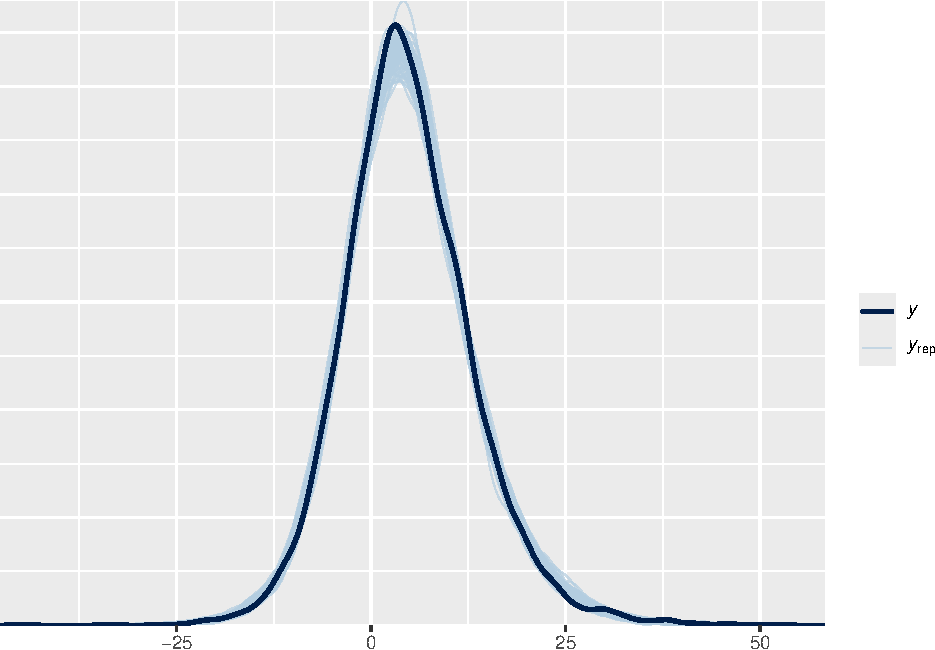
\includegraphics{bachelor_thesis_files/figure-latex/posterior-check-dist-1.pdf}
\caption{\label{fig:posterior-check-dist}Overlay of densities from posterior sample from the distributional model}
\end{figure}

\subsection{Hypothesis Testing}\label{hypothesis-testing}

A primary goal of experiments in cognitive psychology is to test a certain theory. In frequentist analyses this is mostly done using null hypothesis significance testing (NHST). NHST is a way of deciding whither one theory fits the observed data better than a rival one, usually using p-values. This approach has been criticized many times especially for producing non-replicable results (e.g. Halsey et al., 2015; Nickerson, 2000; Szucs \& Ioannidis, 2017). Different solutions, and especially Bayesian analyses, have been proposed to address these issues (e.g. Vandekerckhove et al., 2018; Wagenmakers, 2007). However, even these approaches are criticized by Bayesian statisticians, who say that dichotomous decisions based on a threshold per se cannot represent a complex theory (e.g. McShane et al., 2019).

Nevertheless, as it is standard part of the frequentist framework and almost always reported in ERP studies, the following sections will concentrate on two different approaches to hypothesis testing in Bayesian statistics, Bayes factors (BF) and cross validation. It is important to note here that credible intervals, the Bayesian equivalent to confidence intervals, should not be used to reject or accept a null hypothesis (Wagenmakers et al., 2019). Bayes factors and cross validation come with distinct advantages and drawbacks that will also be discussed. As mentioned before, however, most Bayesian statisticians would advise against dichotomous decisions.

\subsection{Bayes Factors}\label{bayes-factors}

As mentioned above, Bayes Factors are one way to test hypotheses in the Bayesian framework. The BF assesses how well the entire model (prior and likelihood) is able to explain the observed data set relative to another model (Nicenboim et al., n.d.). The model under which the collected data are more likely to occur will be supported by the BF (Wagenmakers et al., 2010). This interpretation is one that is often desired for frequentist hypothesis testing but that NHST cannot provide, so this is one of many advantages of the BF. The BF also allows to collect evidence supporting the null hypothesis, e.g.~when an experiment aims to show the absence of an effect (Wagenmakers et al., 2010).

The Bayes factor is also often criticized, however, and comes with its own challenges (see Tendeiro et al., 2024; Tendeiro \& Kiers, 2019; Vehtari \& Ojanen, 2012). Most importantly, this approach to statistical inference could be seen as not truly Bayesian in the sense that it does not incorporate the entire posterior but rather facilitates a dichotomous decision using a point estimate. In the application, a major challenge in using Bayes factors is their high sensitivity to the prior distributions (Wagenmakers et al., 2010). Also, computations of Bayes factors can be difficult and unstable (Tendeiro \& Kiers, 2019; Wagenmakers et al., 2010) and the interpretation should be treated with caution (Tendeiro \& Kiers, 2019). Despite the drawbacks, Bayes factors can be a useful tool in comparing models and is an improvement over classic NHST (Tendeiro \& Kiers, 2019).

\subsubsection{Mathematical Model and Implementation in R}\label{mathematical-model-and-implementation-in-r-2}

The Bf can be understood and computed by using the marginal likelihood. So far, we have mostly ignored the marginal likelihood, which serves as the denominator in Bayes' rule. For the BF the marginal likelihood is crucial, however. When we aim to compare two competing models, the BF is computed by taking the ratio of the marginal likelihoods under each model (Nicenboim et al., n.d.). In our running example we would like to test whether a model including the fixed slope (\(M_1\)) that represents the experimental effect is more suitable than a model that does not contain that parameter or, equally, assumes it to be zero (\(M_0\)). The BF for this comparison can than be written as in Eq. \eqref{eq:bayes-factor}, by simply including the models into the equation (Gelman et al., 2015).

\begin{equation}
BF_{10} = \frac{p(y|M_1)}{p(y|M_0)} = \frac{\int{p(\theta_1|M_1)p(y_1|\theta_1,M_1)}d\theta_1}{\int{p(\theta_0|M_0)p(y_0|\theta_0,M_0)}d\theta_0}
\label{eq:bayes-factor}
\end{equation}

The basic idea behind the marginal likelihood is that for every possible parameter value, the likelihood is weighted with the corresponding prior (Gelman et al., 2015; Nicenboim et al., n.d.). This product is then integrated over the parameter \(\theta\), i.e.~summed over all possible values of \(\theta\). This shows that even mathematically the prior plays a vital role in the BF. A model that makes better predictions would then yield a higher marginal likelihood.

To calculate the Bayes factor, one then takes the ratio of the two marginal likelihoods. The BF can be interpreted as the relative evidence for the predictive performance of one model over the other (Heck et al., 2023). Specifically it tells us by what amount the observed data are more likely to occur if one model were true compared with the other model being true. Values larger than one support the model \(M_1\), where as values smaller than one support the model \(M_0\), values close to one indicate inconclusive results. Typically, a BF over 10 or under .1 is seen as strong evidence in favor of the first or second model, respectively.

For the implementation in R we will use the bridge sampling method, because it allows to compare non-nested models (e.g. Gronau et al., 2017). Alternatively the Savage--Dickey density ratio method could also be used to compute the BF in R (e.g. Wagenmakers et al., 2010). To get stable estimates when using bridge sampling, it is important to have a large number of effective samples (Gronau et al., 2020). For this reason we will use a greater number of iterations (\texttt{iter\ =\ 20000}), additionally the \texttt{control} parameter is set to \texttt{list(adapt\_delta\ =\ 0.9)} to ensure the sampling process is working properly. It is also necessary to set \texttt{save\_pars\ =\ save\_pars(all\ =\ TRUE)}, this way all the parameters will be saved that are needed to be able to perform bridge sampling. With these adaptations, we will run the \(M_1\) as well as the \(M_0\) model, for the \(M_0\) model, the fixed slope will be excluded. In the following, only the code for the null model is shown.

\begin{Shaded}
\begin{Highlighting}[]
\CommentTok{\# exclude fixed slope beta\_1 in the formula}
\NormalTok{blmm\_bf\_0 }\OtherTok{\textless{}{-}} \FunctionTok{brm}\NormalTok{(N170 }\SpecialCharTok{\textasciitilde{}} \DecValTok{1} \SpecialCharTok{+}\NormalTok{ (}\DecValTok{1} \SpecialCharTok{+}\NormalTok{ f\_c }\SpecialCharTok{|}\NormalTok{ participant\_id),}
                 \AttributeTok{data =}\NormalTok{ trials\_cond, }
                 \CommentTok{\# remove prior for beta\_1}
                 \AttributeTok{prior =}\NormalTok{ prior\_1[prior\_1}\SpecialCharTok{$}\NormalTok{class }\SpecialCharTok{!=} \StringTok{"b"}\NormalTok{, ],}
                 \AttributeTok{warmup =} \DecValTok{2000}\NormalTok{,}
                 \AttributeTok{iter =} \DecValTok{20000}\NormalTok{,}
                 \AttributeTok{cores =} \DecValTok{4}\NormalTok{,}
                 \CommentTok{\# ensure that the sampler is working correctly}
                 \AttributeTok{control =} \FunctionTok{list}\NormalTok{(}\AttributeTok{adapt\_delta =} \FloatTok{0.9}\NormalTok{), }
                 \CommentTok{\# precondition for performing bridge sampling}
                 \AttributeTok{save\_pars =} \FunctionTok{save\_pars}\NormalTok{(}\AttributeTok{all =} \ConstantTok{TRUE}\NormalTok{), }
                 \AttributeTok{family =} \FunctionTok{gaussian}\NormalTok{())}
\end{Highlighting}
\end{Shaded}

After setting up the two alternative models, the marginal log likelihoods are computed using the \texttt{bridge\_sample} function from the bridgesampling package (Version 1.1.2; Gronau et al., 2020). Here, the marginal log likelihoods are used because the marginal likelihoods can be very small in the multidimensional probability space used for sampling and hence can lead to numerical problems.

\begin{Shaded}
\begin{Highlighting}[]
\CommentTok{\# Compute marginal log likelihood for model 1}
\NormalTok{margLogLik\_linear }\OtherTok{\textless{}{-}} \FunctionTok{bridge\_sampler}\NormalTok{(blmm\_bf\_1, }\AttributeTok{silent =} \ConstantTok{TRUE}\NormalTok{)}

\CommentTok{\# Compute marginal log likelihood for model 0}
\NormalTok{margLogLik\_null }\OtherTok{\textless{}{-}} \FunctionTok{bridge\_sampler}\NormalTok{(blmm\_bf\_0, }\AttributeTok{silent =} \ConstantTok{TRUE}\NormalTok{)}
\end{Highlighting}
\end{Shaded}

Finally, these marginal log likelihoods are used to calculate the BF with the \texttt{bayes\_factor} (or \texttt{bf}) function also from the bridgesampling package. The null model is usually last. This way bigger numbers represent evidence for the alternative model.

\begin{Shaded}
\begin{Highlighting}[]
\NormalTok{bf\_blmm }\OtherTok{\textless{}{-}} \FunctionTok{bayes\_factor}\NormalTok{(margLogLik\_linear, margLogLik\_null)}
\end{Highlighting}
\end{Shaded}

\subsubsection{Results}\label{results-3}

For the comparison of the BLMM with and without a fixed slope, the Bayes factor is \(BF_{blmm10} =\) 5,964.87. This means that the observed data are 5965 times more likely to occur if model \(M_1\) (including the fixed slope) were true than if \(M_0\) were true. This can be interpreted as strong evidence for the \(M_1\). In the same way we can compare the distributional model with and without a fixed slope, which gives us a Bayes factor of \(BF_{dist10} =\) 0.04, providing evidence in favour of the null model. When computing Bayes factors with the bridge sampling method, we can also compare non-nested models. The comparison of the standard BLMM and the distributional model returns a Bayes factor of \(BF_{blmm,dist} \approx\) 0, providing very strong evidence that the distributional model fits the data better than the standard BLMM.

\subsubsection{Sensitivity Analysis}\label{sensitivity-analysis}



\begin{figure}
\centering
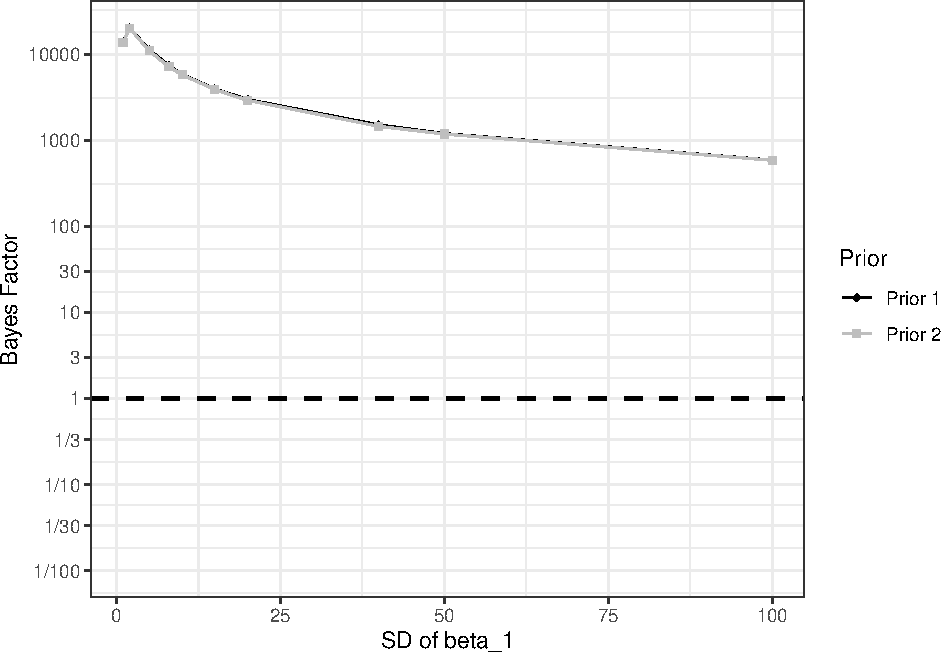
\includegraphics{bachelor_thesis_files/figure-latex/plot-bf-sens-1.pdf}
\caption{\label{fig:plot-bf-sens}Sensitivity Analysis of Bayes Factors for Two Different Priors Depending on Beta\_1 Prior}
\end{figure}

Because the Bayes factor is known to be very sensitive to the priors, it is important to do a sensitivity analysis. In the analysis, you compare the Bayes Factors for different priors to assess how robust your results are. In our case, we will compare two different sets of priors for the BLMM and additionally change the prior of our main fixed effect within each set. The first set of priors is the same we have been using so far and the second set is a wider set of priors, with the standard deviation doubled for each parameter. Only the prior for the correlation \(\rho_u\) is halved (from \texttt{lkj(2)} to \texttt{lkj(1)}) for the distribution to become wider. For \(\beta_1\), we will use ten different standard deviations for each set of priors. Using wider priors that are further away from the true value is a good way to test the robustness of the Bayes factor, because they will usually result in Bayes factors closer to zero. The models are set up in the same way as above, with a null model for each set of priors. Because the main idea stays the same, we will not include the sensitivity analysis for the distributional model here, but it can be found on GitHub. The results of the sensitivity analysis can be found in Fig. \ref{fig:plot-bf-sens}. Regardless of the chosen prior, all the BF in the analysis are at least \(BF_{10} =\) 591.48, which means that the data are 591 times more likely to occur under \(H_1\) than under \(H_0\). This is consistent with the results we have found in Sec. 2.3.3. Additionally, we see little difference between the two sets of priors. These results speak for the robustness of the Bayes factor with regard to the chosen prior.

\subsection{Cross Validation}\label{cross-validation}

The other approach to comparing Bayesian models is cross validation. In contrast to the BF, in cross validation the model is fit only to a subset of the data (training data). The resulting posterior distribution is then used to predict the held-out (or validation) data and the accuracy of the prediction is assessed. This process is repeated several times, until each subset of a partition was left out once. In the following, we will use leave-one-out cross validation (LOO, e.g., Gelman et al., 2014; Vehtari et al., 2017), where the validation data consist only of one data point. Cross validation attempts to assess how our model deals with new data and whether we can generalize to out-of-sample data. Of course the validation data are not actually new, as they were collected with the rest of the data set (Nicenboim et al., n.d.). This approach is less dependent on the prior distribution, especially with the amount of data seen in ERP studies forming the likelihood.

To quantify the accuracy of the prediction, we will use an estimator called expected log pointwise predictive density (\(elpd\)). For each held-out data point the predictive density, given the model and the training data, is calculated. The elpd is obtained by summing over the log of these predictive densities (Gronau \& Wagenmakers, 2019). To compare two models, the difference between the elpd's is computed and the magnitude of this difference is assessed. We will not elaborate on the mathematicel specifics here, but refer the reader to Gelman et al. (2014) and Nicenboim et al. (n.d.) for a detailed introduction to LOO.

For the computation, we use the \texttt{loo} function from the brms package, which builds on the loo package as a backend (Version 2.7.0; Vehtari, Gabry, et al., 2024). It uses Pareto smoothed importance sampling {[}PSIS; Vehtari, Simpson, et al. (2024){]} to compute the \(elpd\). Importance sampling allows to estimate samples from the posterior distribution after removal of one data point without having to re-fit the entire model each time (Vehtari et al., 2017). PSIS is a newer, more stable version of this algorithm providing more reliable and accurate estimates (Vehtari, Simpson, et al., 2024).

The implementation is very straightforward. We first need to calculate the elpd for each model we want to compare. In our case, this means setting up one model with the fixed slope and one null model without this effect. Unlike with BFs, we do not need to increase the iterations because the estimation of the \(elpd\) depends mainly on the number of observations and not the number of samples (Nicenboim et al., n.d.). We only need to set up the null model as in Section 2.10 and then use the \texttt{loo} function for every model. The \texttt{loo} function not only gives us the \texttt{elpd\_loo}, the sum of pointwise predictive accuracy (here a less negative number indicates a better prediction), but also the effective number of parameters \texttt{p\_loo}, an estimate of model complexity, and the LOO information criterion \texttt{looic}, which is just \texttt{-2*elpd\_loo}. Additionally, the function will output some diagnostics. We will not discuss them here, but in general, it is important for a reliable estimation that the Pareto k estimates are small enough (under .7, see Vehtari et al., 2017). After computing the \(elpd\) we can use the \texttt{loo\_compare} function to compare the models. \texttt{loo\_compare} computes the difference between the \(elpd\) of the two models (\texttt{elpd\_diff}) as well as the standard error of this difference (\texttt{se\_diff}). Although these estimates are known to be less sensitive to the priors than the BF, it is nevertheless suggested that a sensitivity analysis be performed for the cross-validation using a few different priors (see Section 2.10.3).

\begin{Shaded}
\begin{Highlighting}[]
\CommentTok{\# Computing the elpd for the standard correlation model}
\NormalTok{loo\_blmm\_1 }\OtherTok{\textless{}{-}} \FunctionTok{loo}\NormalTok{(mod\_blmm)}

\CommentTok{\# Computing the elpd for the null model}
\NormalTok{loo\_blmm\_0 }\OtherTok{\textless{}{-}} \FunctionTok{loo}\NormalTok{(mod\_blmm\_0)}

\CommentTok{\# Comparing the models}
\NormalTok{loo\_comparison\_blmm }\OtherTok{\textless{}{-}} \FunctionTok{loo\_compare}\NormalTok{(loo\_blmm\_1, loo\_blmm\_0)}
\end{Highlighting}
\end{Shaded}

\begin{table}[tbp]

\begin{center}
\begin{threeparttable}

\caption{\label{tab:loo-blmm-table}Comparison of the linear and null BLMM using LOO}

\begin{tabular}{lllllllll}
\toprule
 & \multicolumn{1}{c}{elpd\_diff} & \multicolumn{1}{c}{se\_diff} & \multicolumn{1}{c}{elpd\_loo} & \multicolumn{1}{c}{se\_elpd\_loo} & \multicolumn{1}{c}{p\_loo} & \multicolumn{1}{c}{se\_p\_loo} & \multicolumn{1}{c}{looic} & \multicolumn{1}{c}{se\_looic}\\
\midrule
mod\_blmm & 0.00 & 0.00 & -21,033.57 & 85.90 & 68.91 & 2.08 & 42,067.13 & 171.79\\
mod\_blmm\_0 & -3.53 & 2.70 & -21,037.10 & 85.94 & 75.96 & 2.32 & 42,074.20 & 171.89\\
\bottomrule
\end{tabular}

\end{threeparttable}
\end{center}

\end{table}

\begin{table}[tbp]

\begin{center}
\begin{threeparttable}

\caption{\label{tab:loo-dist-table}Comparison of the linear and null distributional model using LOO}

\begin{tabular}{lllllllll}
\toprule
 & \multicolumn{1}{c}{elpd\_diff} & \multicolumn{1}{c}{se\_diff} & \multicolumn{1}{c}{elpd\_loo} & \multicolumn{1}{c}{se\_elpd\_loo} & \multicolumn{1}{c}{p\_loo} & \multicolumn{1}{c}{se\_p\_loo} & \multicolumn{1}{c}{looic} & \multicolumn{1}{c}{se\_looic}\\
\midrule
mod\_dist & 0.00 & 0.00 & -20,516.24 & 72.28 & 120.45 & 7.50 & 41,032.48 & 144.57\\
mod\_dist\_0 & -3.05 & 2.63 & -20,519.29 & 72.53 & 126.56 & 8.04 & 41,038.59 & 145.05\\
\bottomrule
\end{tabular}

\end{threeparttable}
\end{center}

\end{table}

\begin{table}[tbp]

\begin{center}
\begin{threeparttable}

\caption{\label{tab:loo-blmm-dist-table}Comparison of the BLMM and the distributional model using LOO}

\begin{tabular}{lllllllll}
\toprule
 & \multicolumn{1}{c}{elpd\_diff} & \multicolumn{1}{c}{se\_diff} & \multicolumn{1}{c}{elpd\_loo} & \multicolumn{1}{c}{se\_elpd\_loo} & \multicolumn{1}{c}{p\_loo} & \multicolumn{1}{c}{se\_p\_loo} & \multicolumn{1}{c}{looic} & \multicolumn{1}{c}{se\_looic}\\
\midrule
mod\_dist & 0.00 & 0.00 & -20,516.24 & 72.28 & 120.45 & 7.50 & 41,032.48 & 144.57\\
mod\_blmm & -517.33 & 45.31 & -21,033.57 & 85.90 & 68.91 & 2.08 & 42,067.13 & 171.79\\
\bottomrule
\end{tabular}

\end{threeparttable}
\end{center}

\end{table}

Table \ref{tab:loo-blmm-table} shows the \(elpd\) difference and the se of said difference in the first two columns as well as more detailed information about the models (including \texttt{elpd\_loo}, \texttt{p\_loo} and \texttt{looic}) in the rear columns. An \(elpd\) difference of \(elpd_{diff}\) = -3.50 tells us that the model with the experimental condition as a predictor has a higher predictive accuracy. Although this supports our initial hypothesis, as the difference is smaller than 4 and also smaller than 2 \(se\), it cannot be interpreted as a meaningful superiority of one model over the other (Nicenboim et al., n.d.). The same pattern arises in the comparison of the linear and null distributional model. As we can see in Table \ref{tab:loo-dist-table} the \(elpd_{diff}\) of -3.10 is similarly small. Note that this deviates from the results produced by using BF, where the effect went into the opposite direction for the distributional model. The comparison between the distributional and the standard LMM (see Table \ref{tab:loo-blmm-dist-table}) confirms the strong superiority of the distributional model that we had already seen with the BFs with an \(elpd_{diff}\) of -517.30.

\subsection{Reporting Practices}\label{reporting-practices}

Analyses with BLMMs imply a great amount of researchers' degrees of freedom, and thus it is essential to provide enough information on the analysis for others to be able to reproduce and evaluate it. Simmons et al. (2011) show impressively what can happen when analyses are not disclosed. Ideally, the entire code (and, if possible, data) should be uploaded in an online repository like the Open Science Framework or GitHub (Epskamp, 2019). This not only provides all the analyses in one place but also solves the problem of having to decide what to report within a possibly limited word count. In addition, if the analyses were conducted in R researchers could consider making it entirely reproducible (see e.g., Brandmaier \& Peikert, 2024; Marwick et al., 2018; Peikert \& Brandmaier, 2019).

Generally, the software used for the analyses should be cited as well as all associated packages with version numbers, respectively. Epskamp (2019) even suggests to use a package like renv (Version 1.0.7; \textbf{R-renv?}) that stores the source code of every package at the point of use and makes later reproducibility much easier. Also, setting a seed for the generation of pseudorandom numbers at the beginning of the analysis helps with more exact reproducibility. The variables (dependent and independent) and hypotheses should be clearly named and explained further if necessary (Kruschke, 2021; van Doorn et al., 2021). It might also be helpful, to explain why one chose a specific method and explain the method and possible benefits if the audience requires it (Kruschke, 2021). Additionally, for different methods different aspects might be reported (e.g.~inclusion criteria for a meta-analysis Hansen et al., 2022). We will discuss the primary reporting practices for LMMs and Bayesian methods next.

For frequentist LMMs Meteyard and Davies (2020) provide a comprehensive overview on reporting practices. They recommend to report the equation of the final model as well as the approach used for model selection. Reporting additional models (not only the final one) can also be beneficial (Wagenmakers et al., 2021). Meteyard and Davies (2020) also suggest to provide point estimates, standard errors, and confidence intervals of the fixed effects and all variances of random effects. If p values are used, the method to approximate degrees of freedom should be stated (Meteyard \& Davies, 2020).

In Bayesian statistics reporting becomes even more important due to the increased researchers' degrees of freedom but also more complicated because among other things we are dealing with posterior distributions, not only point estimates. Depending on the performed analysis, very different things should be reported in papers using Bayesian methods. In the following we will concentrate on the most important aspects for the analyses performed above. Kruschke (2021) gives a more detailed review on Bayesian reporting practices and guidelines to improve reproducibility and quality of Bayesian analyses.

As part of the methods presentation the assumed likelihood function should be explained, the prior distributions should be stated and justified for each parameter and the model should be formally specified (include likelihood and prior) (Kruschke, 2021). For multilevel models, like the ones discussed in this paper, the hierarchical structure should be explained. Kruschke (2021) recommends performing and reporting prior predictive checks (see Section 2.5), especially for more informative priors. The performance of the computation (MCMC in our case) should also be reported, here Kruschke (2021) recommends to report a convergence measure, like the \(\hat{R}\) seen above, and a measure for the resolution, this refers to the ESS. Since MCMC algorithms can be quite time-intensive it might be advised to publish the entire MCMC chain. The posterior distributions should be summarized by a measure of central tendency and the credible interval, ideally, posterior predictive checks should show that the model mimics the data (Kruschke, 2021). For hypothesis testing, Kruschke (2021) suggests to state the decision procedure/threshold and the observed BF and posterior probabilities or the observed difference in elpd. Finally, the sensitivity analysis should be reported to show whether or how the prior influences the posterior and especially whether the decisions change under different priors (Kruschke, 2021; van Doorn et al., 2021). Ideally, this should include a plot as well as a numerical report of the results (van Doorn et al., 2021). Of course, additional analysis might need further reporting and researchers might choose to address some of the points discussed in the appendix or supplementary material.

\section{Discussion}\label{discussion}

\subsection{Advantages and Disadvantages of Bayesian Linear Mixed Models}\label{advantages-and-disadvantages-of-bayesian-linear-mixed-models}

Bayesian methods have become increasingly popular in the cognitive sciences (e.g., Lee, 2011). In the course of this tutorial, we have seen some advantages and disadvantages of this approach in a practical application using Bayesian LMMs. BLMMs account for the nested structure of EEG data in the same way as frequentist LMMs, while at the same time incorporating the Bayesian framework. This framework, while needing some familiarization in the beginning, makes it possible to flexibly adapt to the intricacies of the data at hand (Bürkner, 2018; Kruschke, 2021). As we have seen with the distributional regression, an extension to more complex models can easily be incorporated (see Section 2.8.1). Distributional modeling has significantly improved model fit by accounting for the noise variance across participants. This offered improved prediction capabilities and emphasised a benefit over frequentist methods, which must assume homogeneity in residual variances. The Bayesian framework also allows to quantify the uncertainty of the estimation by relying on probability distributions instead of point estimates (Section 2.3.1). Another major advantage lies in Bayesian hypothesis testing, which allows evidence collection both for and against the null hypothesis, whilst also addressing some limitations of the frequentist NHST widely used in EEG research. Both Bayes factors and cross validation were used for model comparison. The common assumption that Bayes factors are highly sensitive to the chosen priors (e.g. Wagenmakers et al., 2010) was not apparent in our data, which might make BFs especially suitable for ERP studies with many data points.

Despite these advantages, Bayesian methods do also present with some challenges. One significant limitation is the computational power needed. Especially for complex models with numerous parameters the Bayesian sampling methods like MCMC can require substantial computation time, with even increased recourses needed for computing Bayes factors. The sensitivity analysis for the BFs in Section 2.10.3 run on a MacBook Air with a 3.49 GHz M2 chip with 16 GB RAM took several hours. Another limitation is the reliance on appropriate priors, which can be difficult to determine in studies with novel designs. Although the Bayes factor (and analysis in general) did not significantly vary in our analysis, data sets with less data points might be more sensitive to unsuitable priors. As there is little knowledge for prior elicitation available so far, this can still pose a problem. A major probelm were also the diverging results of the model comparison. The results of the cross validation went into the expected direction, but were too small to be interpreted meaningfully, reflecting a problem of the cross validation with small effects that has already been discussed (Sivula et al., 2022). The Bayes factors even showed opposing effects in the distributional regression. Only the superiority of the distributional model was consistent in both analyses. This raises the question, how model comparison should best be approached for EEG data. Additionally, because a cut-off is used for interpretation, BFs are often regarded as not truly Bayesian. Ideally, the BF should therfore be combined with prior odds but those are very difficult to find out because we do not know the prior probability of a model (Tendeiro \& Kiers, 2019). Finally, while the amount of decisions preciding the statistical analysis is already high for frequentist linear mixed models (Brown, 2021), for Bayesian methods the amount gets considerably bigger. This makes adequate reporting and transperancy even more important (see Kruschke, 2021; Meteyard \& Davies, 2020; van Doorn et al., 2021) and should always be considered by researchers using Bayesian methods.

\subsection{Limitations of the Present Study and Further Research}\label{limitations-of-the-present-study-and-further-research}

Due to the introductory nature of this tutorial, many topics could not be presented in depth. So far we have, for example, only looked at very simple hypotheses including only one predictor and only the participants as random effects. To be able to address more differentiated research questions, it is necessary to extend the structure of the mixed models. This expansion could include additional predictors, interactions, and crossed random effects. An important question would be, whether existing recommendations regarding the model specification (e.g. Barr et al., 2013; Bates et al., 2018; Bürki et al., 2018; Judd et al., 2012; Matuschek et al., 2017) also hold for BLMMs and wether similar priors work similarly well. It would also be crucial to look at the effects of model extensions on computation time, convergence, model comparison and how the priors influence those effects.

Addtionally, this tutorial did not include testing the assumptions underlying the statistical methods. In traditional mixed models, assumptions such as linearity, normal distribution of residual errors and random effect deviations, and homoscedasticity are critical for model validity (e.g. Field \& Wright, 2011; Maas \& Hox, 2004). Practical approaches for assumption checking, such as plotting residuals and random effects, can offer visual insights into model fit (e.g. Winter, 2013).

Finally, the methods for model comparison should be investigated further. It is still unclear why the main effect disappears when Bayes factors are used for the distributional model and why there is a difference in the magnitude of the evidence between BF and cross validation in the standard BLMM. For future use of Bayesian model comparison methods, it is important to assess whether these findings translate to other ERP components and data sets and what recommendations could be made regarding these issues.

The present tutorial only represents the very beginning of using Bayesian methods in the statistical analysis of ERP studies. Many additional points should be considered in further research. Especially important would be the extension to multiple predictors and crossed random effects as well as giving a rationale for model choice that includes the challenges we have encountered here. Additionaly, it would be of interest to assess whether the priors used here could serve as a starting point for ERP components in general. All of this could help introduce Bayesian methods as a more widely used analysis in ERP research.

\newpage

\section{References}\label{references}

\phantomsection\label{refs}
\begin{CSLReferences}{1}{0}
\bibitem[\citeproctext]{ref-baayen_etal08}
Baayen, R. H., Davidson, D. J., \& Bates, D. M. (2008). Mixed-effects modeling with crossed random effects for subjects and items. \emph{Journal of Memory and Language}, \emph{59}(4), 390--412. \url{https://doi.org/10.1016/j.jml.2007.12.005}

\bibitem[\citeproctext]{ref-bagiella_etal00}
Bagiella, E., Sloan, R. P., \& Heitjan, D. F. (2000). Mixed-effects models in psychophysiology. \emph{Psychophysiology}, \emph{37}(1), 13--20. \url{https://doi.org/10.1111/1469-8986.3710013}

\bibitem[\citeproctext]{ref-barr_etal13}
Barr, D. J., Levy, R., Scheepers, C., \& Tily, H. J. (2013). Random effects structure for confirmatory hypothesis testing: {Keep} it maximal. \emph{Journal of Memory and Language}, \emph{68}(3), 255--278. \url{https://doi.org/10.1016/j.jml.2012.11.001}

\bibitem[\citeproctext]{ref-bates_etal18}
Bates, D., Kliegl, R., Vasishth, S., \& Baayen, H. (2018, May 26). \emph{Parsimonious {Mixed Models}}. \url{https://doi.org/10.48550/arXiv.1506.04967}

\bibitem[\citeproctext]{ref-betancourt18}
Betancourt, M. (2018, July 15). \emph{A {Conceptual Introduction} to {Hamiltonian Monte Carlo}}. \url{http://arxiv.org/abs/1701.02434}

\bibitem[\citeproctext]{ref-brandmaier_peikert24}
Brandmaier, A. M., \& Peikert, A. (2024, June 27). \emph{Automated {Reproducibility Testing} in {R Markdown}}. \url{https://doi.org/10.31234/osf.io/3zjvf}

\bibitem[\citeproctext]{ref-brauer_curtin18}
Brauer, M., \& Curtin, J. J. (2018). Linear mixed-effects models and the analysis of nonindependent data: {A} unified framework to analyze categorical and continuous independent variables that vary within-subjects and/or within-items. \emph{Psychological Methods}, \emph{23}(3), 389--411. \url{https://doi.org/10.1037/met0000159}

\bibitem[\citeproctext]{ref-brown21}
Brown, V. A. (2021). An {Introduction} to {Linear Mixed-Effects Modeling} in {R}. \emph{Advances in Methods and Practices in Psychological Science}, \emph{4}(1), 2515245920960351. \url{https://doi.org/10.1177/2515245920960351}

\bibitem[\citeproctext]{ref-burki_etal18}
Bürki, A., Frossard, J., \& Renaud, O. (2018). Accounting for stimulus and participant effects in event-related potential analyses to increase the replicability of studies. \emph{Journal of Neuroscience Methods}, \emph{309}, 218--227. \url{https://doi.org/10.1016/j.jneumeth.2018.09.016}

\bibitem[\citeproctext]{ref-burkner18}
Bürkner, P.-C. (2018). Advanced {Bayesian Multilevel Modeling} with the {R Package} brms. \emph{The R Journal}, \emph{10}(1), 395. \url{https://doi.org/10.32614/RJ-2018-017}

\bibitem[\citeproctext]{ref-burkner24}
Bürkner, P.-C. (2024, March 19). \emph{Estimating {Distributional Models} with brms}. \url{https://cran.r-project.org/web/packages/brms/vignettes/brms_distreg.html}

\bibitem[\citeproctext]{ref-carpenter_etal17}
Carpenter, B., Gelman, A., Hoffman, M. D., Lee, D., Goodrich, B., Betancourt, M., Brubaker, M., Guo, J., Li, P., \& Riddell, A. (2017). \emph{Stan} : {A Probabilistic Programming Language}. \emph{Journal of Statistical Software}, \emph{76}(1). \url{https://doi.org/10.18637/jss.v076.i01}

\bibitem[\citeproctext]{ref-depaoli_etal17}
Depaoli, S., Rus, H. M., Clifton, J. P., van de Schoot, R., \& Tiemensma, J. (2017). An introduction to {Bayesian} statistics in health psychology. \emph{Health Psychology Review}, \emph{11}(3), 248--264. \url{https://doi.org/10.1080/17437199.2017.1343676}

\bibitem[\citeproctext]{ref-eimer11a}
Eimer, M. (2011). The {Face-Sensitivity} of the {N170 Component}. \emph{Frontiers in Human Neuroscience}, \emph{5}, 119. \url{https://doi.org/10.3389/fnhum.2011.00119}

\bibitem[\citeproctext]{ref-enge_etal23}
Enge, A., Süß, F., \& Rahman, R. A. (2023). Instant {Effects} of {Semantic Information} on {Visual Perception}. \emph{Journal of Neuroscience}, \emph{43}(26), 4896--4906. \url{https://doi.org/10.1523/JNEUROSCI.2038-22.2023}

\bibitem[\citeproctext]{ref-epskamp19}
Epskamp, S. (2019). Reproducibility and {Replicability} in a {Fast-Paced Methodological World}. \emph{Advances in Methods and Practices in Psychological Science}, \emph{2}(2), 145--155. \url{https://doi.org/10.1177/2515245919847421}

\bibitem[\citeproctext]{ref-field_wright11}
Field, A. P., \& Wright, D. B. (2011). A {Primer} on {Using Multilevel Models} in {Clinical} and {Experimental Psychopathology Research}. \emph{Journal of Experimental Psychopathology}, \emph{2}(2), 271--293. \url{https://doi.org/10.5127/jep.013711}

\bibitem[\citeproctext]{ref-fromer_etal18}
Frömer, R., Maier, M., \& Abdel Rahman, R. (2018). Group-level {EEG-processing} pipeline for flexible single trial-based analyses including linear mixed models. \emph{Frontiers in Neuroscience}, \emph{12}. \url{https://www.frontiersin.org/articles/10.3389/fnins.2018.00048}

\bibitem[\citeproctext]{ref-gelmana}
Gelman, A. (n.d.). \emph{When {MCMC} fails: {The} advice we're giving is wrong. {Here}'s what we you should be doing instead. ({Hint}: It's all about the folk theorem.) \textbar{} {Statistical Modeling}, {Causal Inference}, and {Social Science}}. Retrieved October 29, 2024, from \url{https://statmodeling.stat.columbia.edu/2021/06/10/when-mcmc-fails-the-advice-were-giving-is-wrong-heres-what-we-you-should-be-doing-instead-hint-its-all-about-the-folk-theorem/}

\bibitem[\citeproctext]{ref-gelman_etal15}
Gelman, A., Carlin, J. B., Stern, H. S., Dunson, D. B., Vehtari, A., \& Rubin, D. B. (2015). \emph{Bayesian {Data Analysis}} (3rd ed.). {Chapman and Hall/CRC}. \url{https://doi.org/10.1201/b16018}

\bibitem[\citeproctext]{ref-gelman_etal14}
Gelman, A., Hwang, J., \& Vehtari, A. (2014). Understanding predictive information criteria for {Bayesian} models. \emph{Statistics and Computing}, \emph{24}(6), 997--1016. \url{https://doi.org/10.1007/s11222-013-9416-2}

\bibitem[\citeproctext]{ref-gelman_etal17}
Gelman, A., Simpson, D., \& Betancourt, M. (2017). The {Prior Can Often Only Be Understood} in the {Context} of the {Likelihood}. \emph{Entropy}, \emph{19}(10, 10), 555. \url{https://doi.org/10.3390/e19100555}

\bibitem[\citeproctext]{ref-gronau_etal17}
Gronau, Q. F., Sarafoglou, A., Matzke, D., Ly, A., Boehm, U., Marsman, M., Leslie, D. S., Forster, J. J., Wagenmakers, E.-J., \& Steingroever, H. (2017). A tutorial on bridge sampling. \emph{Journal of Mathematical Psychology}, \emph{81}, 80--97. \url{https://doi.org/10.1016/j.jmp.2017.09.005}

\bibitem[\citeproctext]{ref-gronau_etal20}
Gronau, Q. F., Singmann, H., \& Wagenmakers, E.-J. (2020). Bridgesampling: {An R Package} for {Estimating Normalizing Constants}. \emph{Journal of Statistical Software}, \emph{92}, 1--29. \url{https://doi.org/10.18637/jss.v092.i10}

\bibitem[\citeproctext]{ref-gronau_wagenmakers19}
Gronau, Q. F., \& Wagenmakers, E.-J. (2019). Limitations of {Bayesian Leave-One-Out Cross-Validation} for {Model Selection}. \emph{Computational Brain \& Behavior}, \emph{2}(1), 1--11. \url{https://doi.org/10.1007/s42113-018-0011-7}

\bibitem[\citeproctext]{ref-halsey_etal15}
Halsey, L. G., Curran-Everett, D., Vowler, S. L., \& Drummond, G. B. (2015). The fickle {P} value generates irreproducible results. \emph{Nature Methods}, \emph{12}(3), 179--185. \url{https://doi.org/10.1038/nmeth.3288}

\bibitem[\citeproctext]{ref-hansen_etal22}
Hansen, C., Steinmetz, H., \& Block, J. (2022). How to conduct a meta-analysis in eight steps: A practical guide. \emph{Management Review Quarterly}, \emph{72}(1), 1--19. \url{https://doi.org/10.1007/s11301-021-00247-4}

\bibitem[\citeproctext]{ref-heck_etal23}
Heck, D. W., Boehm, U., Böing-Messing, F., Bürkner, P.-C., Derks, K., Dienes, Z., Fu, Q., Gu, X., Karimova, D., Kiers, H. A. L., Klugkist, I., Kuiper, R. M., Lee, M. D., Leenders, R., Leplaa, H. J., Linde, M., Ly, A., Meijerink-Bosman, M., Moerbeek, M., \ldots{} Hoijtink, H. (2023). A review of applications of the {Bayes} factor in psychological research. \emph{Psychological Methods}, \emph{28}(3), 558--579. \url{https://doi.org/10.1037/met0000454}

\bibitem[\citeproctext]{ref-itier_taylor04}
Itier, R. J., \& Taylor, M. J. (2004). N170 or {N1}? {Spatiotemporal Differences} between {Object} and {Face Processing Using ERPs}. \emph{Cerebral Cortex}, \emph{14}(2), 132--142. \url{https://doi.org/10.1093/cercor/bhg111}

\bibitem[\citeproctext]{ref-joe06}
Joe, H. (2006). Generating random correlation matrices based on partial correlations. \emph{Journal of Multivariate Analysis}, \emph{97}(10), 2177--2189. \url{https://doi.org/10.1016/j.jmva.2005.05.010}

\bibitem[\citeproctext]{ref-judd_etal12}
Judd, C. M., Westfall, J., \& Kenny, D. A. (2012). Treating stimuli as a random factor in social psychology: A new and comprehensive solution to a pervasive but largely ignored problem. \emph{Journal of Personality and Social Psychology}, \emph{103}(1), 54--69. \url{https://doi.org/10.1037/a0028347}

\bibitem[\citeproctext]{ref-kappenman_etal21}
Kappenman, E. S., Farrens, J. L., Zhang, W., Stewart, A. X., \& Luck, S. J. (2021). {ERP CORE}: {An} open resource for human event-related potential research. \emph{NeuroImage}, \emph{225}, 117465. \url{https://doi.org/10.1016/j.neuroimage.2020.117465}

\bibitem[\citeproctext]{ref-klein24}
Klein, N. (2024). Distributional {Regression} for {Data Analysis}. \emph{Annual Review of Statistics and Its Application}, \emph{11}, 321--346. \url{https://doi.org/10.1146/annurev-statistics-040722-053607}

\bibitem[\citeproctext]{ref-kneib_etal23}
Kneib, T., Silbersdorff, A., \& Säfken, B. (2023). Rage {Against} the {Mean} -- {A Review} of {Distributional Regression Approaches}. \emph{Econometrics and Statistics}, \emph{26}, 99--123. \url{https://doi.org/10.1016/j.ecosta.2021.07.006}

\bibitem[\citeproctext]{ref-kruschke21}
Kruschke, J. K. (2021). Bayesian {Analysis Reporting Guidelines}. \emph{Nature Human Behaviour}, \emph{5}(10), 1282--1291. \url{https://doi.org/10.1038/s41562-021-01177-7}

\bibitem[\citeproctext]{ref-R-lmerTest}
Kuznetsova, A., Brockhoff, P. B., \& Christensen, R. H. B. (2017a). {lmerTest} package: Tests in linear mixed effects models. \emph{Journal of Statistical Software}, \emph{82}(13), 1--26. \url{https://doi.org/10.18637/jss.v082.i13}

\bibitem[\citeproctext]{ref-kuznetsova_etal17}
Kuznetsova, A., Brockhoff, P. B., \& Christensen, R. H. B. (2017b). {lmerTest Package}: {Tests} in {Linear Mixed Effects Models}. \emph{Journal of Statistical Software}, \emph{82}, 1--26. \url{https://doi.org/10.18637/jss.v082.i13}

\bibitem[\citeproctext]{ref-lee11}
Lee, M. D. (2011). How cognitive modeling can benefit from hierarchical {Bayesian} models. \emph{Journal of Mathematical Psychology}, \emph{55}(1), 1--7. \url{https://doi.org/10.1016/j.jmp.2010.08.013}

\bibitem[\citeproctext]{ref-lee_vanpaemel18}
Lee, M. D., \& Vanpaemel, W. (2018). Determining informative priors for cognitive models. \emph{Psychonomic Bulletin \& Review}, \emph{25}(1), 114--127. \url{https://doi.org/10.3758/s13423-017-1238-3}

\bibitem[\citeproctext]{ref-lewandowski_etal09}
Lewandowski, D., Kurowicka, D., \& Joe, H. (2009). Generating random correlation matrices based on vines and extended onion method. \emph{Journal of Multivariate Analysis}, \emph{100}(9), 1989--2001. \url{https://doi.org/10.1016/j.jmva.2009.04.008}

\bibitem[\citeproctext]{ref-maas_hox04}
Maas, C. J. M., \& Hox, J. J. (2004). The influence of violations of assumptions on multilevel parameter estimates and their standard errors. \emph{Computational Statistics \& Data Analysis}, \emph{46}(3), 427--440. \url{https://doi.org/10.1016/j.csda.2003.08.006}

\bibitem[\citeproctext]{ref-marwick_etal18}
Marwick, B., Boettiger, C., \& Mullen, L. (2018). Packaging {Data Analytical Work Reproducibly Using R} (and {Friends}). \emph{The American Statistician}, \emph{72}(1), 80--88. \url{https://doi.org/10.1080/00031305.2017.1375986}

\bibitem[\citeproctext]{ref-matuschek_etal17}
Matuschek, H., Kliegl, R., Vasishth, S., Baayen, H., \& Bates, D. (2017). Balancing {Type I} error and power in linear mixed models. \emph{Journal of Memory and Language}, \emph{94}, 305--315. \url{https://doi.org/10.1016/j.jml.2017.01.001}

\bibitem[\citeproctext]{ref-mcshane_etal19}
McShane, B. B., Gal, D., Gelman, A., Robert, C., \& Tackett, J. L. (2019). Abandon {Statistical Significance}. \emph{The American Statistician}, \emph{73}, 235--245. \url{https://doi.org/10.1080/00031305.2018.1527253}

\bibitem[\citeproctext]{ref-meteyard_davies20}
Meteyard, L., \& Davies, R. A. I. (2020). Best practice guidance for linear mixed-effects models in psychological science. \emph{Journal of Memory and Language}, \emph{112}, 104092. \url{https://doi.org/10.1016/j.jml.2020.104092}

\bibitem[\citeproctext]{ref-mikkola_etal23}
Mikkola, P., Martin, O. A., Chandramouli, S., Hartmann, M., Pla, O. A., Thomas, O., Pesonen, H., Corander, J., Vehtari, A., Kaski, S., Bürkner, P.-C., \& Klami, A. (2023). Prior {Knowledge Elicitation}: {The Past}, {Present}, and {Future}. \emph{Bayesian Analysis}, \emph{-1}, 1--33. \url{https://doi.org/10.1214/23-BA1381}

\bibitem[\citeproctext]{ref-nan_etal22}
Nan, W., Liu, Y., Zeng, X., Yang, W., Liang, J., Lan, Y., \& Fu, S. (2022). The spatiotemporal characteristics of {N170s} for faces and words: {A} meta-analysis study. \emph{PsyCh Journal}, \emph{11}(1), 5--17. \url{https://doi.org/10.1002/pchj.511}

\bibitem[\citeproctext]{ref-nelder_wedderburn72}
Nelder, J. A., \& Wedderburn, R. W. M. (1972). Generalized {Linear Models}. \emph{Journal of the Royal Statistical Society. Series A (General)}, \emph{135}(3), 370--384. \url{https://doi.org/10.2307/2344614}

\bibitem[\citeproctext]{ref-nicenboim_etal}
Nicenboim, B., Schad, D., \& Vasishth, S. (n.d.). \emph{An {Introduction} to {Bayesian Data Analysis} for {Cognitive Science}}. Retrieved June 17, 2024, from \url{https://vasishth.github.io/bayescogsci/book/}

\bibitem[\citeproctext]{ref-nickerson00}
Nickerson, R. S. (2000). Null hypothesis significance testing: {A} review of an old and continuing controversy. \emph{Psychological Methods}, \emph{5}(2), 241--301. \url{https://doi.org/10.1037/1082-989X.5.2.241}

\bibitem[\citeproctext]{ref-nieuwland_etal18}
Nieuwland, M. S., Politzer-Ahles, S., Heyselaar, E., Segaert, K., Darley, E., Kazanina, N., Von Grebmer Zu Wolfsthurn, S., Bartolozzi, F., Kogan, V., Ito, A., Mézière, D., Barr, D. J., Rousselet, G. A., Ferguson, H. J., Busch-Moreno, S., Fu, X., Tuomainen, J., Kulakova, E., Husband, E. M., \ldots{} Huettig, F. (2018). Large-scale replication study reveals a limit on probabilistic prediction in language comprehension. \emph{eLife}, \emph{7}, e33468. \url{https://doi.org/10.7554/eLife.33468}

\bibitem[\citeproctext]{ref-peikert_brandmaier19}
Peikert, A., \& Brandmaier, A. M. (2019). \emph{A {Reproducible Data Analysis Workflow} with {R Markdown}, {Git}, {Make}, and {Docker}}. \url{https://doi.org/10.31234/osf.io/8xzqy}

\bibitem[\citeproctext]{ref-picton_etal00}
Picton, T. w., Bentin, S., Berg, P., Donchin, E., Hillyard, S. a., Johnson JR., R., Miller, G. a., Ritter, W., Ruchkin, D. s., Rugg, M. d., \& Taylor, M. j. (2000). Guidelines for using human event-related potentials to study cognition: {Recording} standards and publication criteria. \emph{Psychophysiology}, \emph{37}(2), 127--152. \url{https://doi.org/10.1111/1469-8986.3720127}

\bibitem[\citeproctext]{ref-roberts_pashler00}
Roberts, S., \& Pashler, H. (2000). How persuasive is a good fit? {A} comment on theory testing. \emph{Psychological Review}, \emph{107}(2), 358--367. \url{https://doi.org/10.1037/0033-295X.107.2.358}

\bibitem[\citeproctext]{ref-roy20}
Roy, V. (2020). Convergence {Diagnostics} for {Markov Chain Monte Carlo}. \emph{Annual Review of Statistics and Its Application}, \emph{7}, 387--412. \url{https://doi.org/10.1146/annurev-statistics-031219-041300}

\bibitem[\citeproctext]{ref-shiffrin_etal08}
Shiffrin, R. M., Lee, M. D., Kim, W., \& Wagenmakers, E.-J. (2008). A {Survey} of {Model Evaluation Approaches With} a {Tutorial} on {Hierarchical Bayesian Methods}. \emph{Cognitive Science}, \emph{32}(8), 1248--1284. \url{https://doi.org/10.1080/03640210802414826}

\bibitem[\citeproctext]{ref-simmons_etal11}
Simmons, J. P., Nelson, L. D., \& Simonsohn, U. (2011). False-{Positive Psychology}: {Undisclosed Flexibility} in {Data Collection} and {Analysis Allows Presenting Anything} as {Significant}. \emph{Psychological Science}, \emph{22}(11), 1359--1366. \url{https://doi.org/10.1177/0956797611417632}

\bibitem[\citeproctext]{ref-sivula_etal22}
Sivula, T., Magnusson, M., Matamoros, A. A., \& Vehtari, A. (2022, March 17). \emph{Uncertainty in {Bayesian Leave-One-Out Cross-Validation Based Model Comparison}}. \url{http://arxiv.org/abs/2008.10296}

\bibitem[\citeproctext]{ref-sorensen_etal16}
Sorensen, T., Hohenstein, S., \& Vasishth, S. (2016). Bayesian linear mixed models using {Stan}: {A} tutorial for psychologists, linguists, and cognitive scientists. \emph{The Quantitative Methods for Psychology}, \emph{12}(3), 175--200. \url{https://doi.org/10.20982/tqmp.12.3.p175}

\bibitem[\citeproctext]{ref-standevelopmentteam24}
Stan Development Team. (2024). \emph{Stan {Modeling Language Users Guide} and {Reference Manual}} (Version 2.35). \url{https://mc-stan.org}

\bibitem[\citeproctext]{ref-szucs_ioannidis17}
Szucs, D., \& Ioannidis, J. P. A. (2017). When {Null Hypothesis Significance Testing Is Unsuitable} for {Research}: {A Reassessment}. \emph{Frontiers in Human Neuroscience}, \emph{11}. \url{https://doi.org/10.3389/fnhum.2017.00390}

\bibitem[\citeproctext]{ref-tendeiro_kiers19}
Tendeiro, J. N., \& Kiers, H. A. L. (2019). A review of issues about null hypothesis {Bayesian} testing. \emph{Psychological Methods}, \emph{24}(6), 774--795. \url{https://doi.org/10.1037/met0000221}

\bibitem[\citeproctext]{ref-tendeiro_etal24}
Tendeiro, J. N., Kiers, H. A. L., Hoekstra, R., Wong, T. K., \& Morey, R. D. (2024). Diagnosing the {Misuse} of the {Bayes Factor} in {Applied Research}. \emph{Advances in Methods and Practices in Psychological Science}, \emph{7}(1), 25152459231213371. \url{https://doi.org/10.1177/25152459231213371}

\bibitem[\citeproctext]{ref-tibon_levy15}
Tibon, R., \& Levy, D. A. (2015). Striking a balance: Analyzing unbalanced event-related potential data. \emph{Frontiers in Psychology}, \emph{6}. \url{https://doi.org/10.3389/fpsyg.2015.00555}

\bibitem[\citeproctext]{ref-vandeschoot_etal21}
van de Schoot, R., Depaoli, S., King, R., Kramer, B., Märtens, K., Tadesse, M. G., Vannucci, M., Gelman, A., Veen, D., Willemsen, J., \& Yau, C. (2021). Bayesian statistics and modelling. \emph{Nature Reviews Methods Primers}, \emph{1}(1), 1--26. \url{https://doi.org/10.1038/s43586-020-00001-2}

\bibitem[\citeproctext]{ref-vandoorn_etal21}
van Doorn, J., van den Bergh, D., Böhm, U., Dablander, F., Derks, K., Draws, T., Etz, A., Evans, N. J., Gronau, Q. F., Haaf, J. M., Hinne, M., Kucharský, Š., Ly, A., Marsman, M., Matzke, D., Gupta, A. R. K. N., Sarafoglou, A., Stefan, A., Voelkel, J. G., \& Wagenmakers, E.-J. (2021). The {JASP} guidelines for conducting and reporting a {Bayesian} analysis. \emph{Psychonomic Bulletin \& Review}, \emph{28}(3), 813--826. \url{https://doi.org/10.3758/s13423-020-01798-5}

\bibitem[\citeproctext]{ref-vandekerckhove_etal18}
Vandekerckhove, J., Rouder, J. N., \& Kruschke, J. K. (2018). Editorial: {Bayesian} methods for advancing psychological science. \emph{Psychonomic Bulletin \& Review}, \emph{25}(1), 1--4. \url{https://doi.org/10.3758/s13423-018-1443-8}

\bibitem[\citeproctext]{ref-vehtari_etal24a}
Vehtari, A., Gabry, J., Magnusson, M., Yao, Y., Bürkner, P.-C., Paananen, T., Gelman, A., Goodrich, B., Piironen, J., Nicenboim, B., \& Lindgren, L. (2024). \emph{Loo: {Efficient Leave-One-Out Cross-Validation} and {WAIC} for {Bayesian Models}} (Version 2.8.0). \url{https://cran.r-project.org/web/packages/loo/index.html}

\bibitem[\citeproctext]{ref-vehtari_etal17}
Vehtari, A., Gelman, A., \& Gabry, J. (2017). Practical {Bayesian} model evaluation using leave-one-out cross-validation and {WAIC}. \emph{Statistics and Computing}, \emph{27}(5), 1413--1432. \url{https://doi.org/10.1007/s11222-016-9696-4}

\bibitem[\citeproctext]{ref-vehtari_etal21}
Vehtari, A., Gelman, A., Simpson, D., Carpenter, B., \& Bürkner, P.-C. (2021). Rank-{Normalization}, {Folding}, and {Localization}: {An Improved Rˆ} for {Assessing Convergence} of {MCMC} (with {Discussion}). \emph{Bayesian Analysis}, \emph{16}(2), 667--718. \url{https://doi.org/10.1214/20-BA1221}

\bibitem[\citeproctext]{ref-vehtari_ojanen12}
Vehtari, A., \& Ojanen, J. (2012). A survey of {Bayesian} predictive methods for model assessment, selection and comparison. \emph{Statistics Surveys}, \emph{6}, 142--228. \url{https://doi.org/10.1214/12-SS102}

\bibitem[\citeproctext]{ref-vehtari_etal24}
Vehtari, A., Simpson, D., Gelman, A., Yao, Y., \& Gabry, J. (2024). Pareto {Smoothed Importance Sampling}. \emph{Journal of Machine Learning Research}, \emph{25}(72), 1--58. \url{http://jmlr.org/papers/v25/19-556.html}

\bibitem[\citeproctext]{ref-volpert-esmond_etal21}
Volpert-Esmond, H. I., Page-Gould, E., \& Bartholow, B. D. (2021). Using multilevel models for the analysis of event-related potentials. \emph{International Journal of Psychophysiology}, \emph{162}, 145--156. \url{https://doi.org/10.1016/j.ijpsycho.2021.02.006}

\bibitem[\citeproctext]{ref-wagenmakers07}
Wagenmakers, E.-J. (2007). A practical solution to the pervasive problems of p values. \emph{Psychonomic Bulletin \& Review}, \emph{14}(5), 779--804. \url{https://doi.org/10.3758/BF03194105}

\bibitem[\citeproctext]{ref-wagenmakers_etal19}
Wagenmakers, E.-J., Lee, M., Rouder, J. N., \& Morey, R. D. (2019, June 6). \emph{The {Principle} of {Predictive Irrelevance}, or {Why Intervals Should Not} be {Used} for {Model Comparison Featuring} a {Point Null Hypothesis}}. \url{https://doi.org/10.31234/osf.io/rqnu5}

\bibitem[\citeproctext]{ref-wagenmakers_etal10}
Wagenmakers, E.-J., Lodewyckx, T., Kuriyal, H., \& Grasman, R. (2010). Bayesian hypothesis testing for psychologists: {A} tutorial on the {Savage}--{Dickey} method. \emph{Cognitive Psychology}, \emph{60}(3), 158--189. \url{https://doi.org/10.1016/j.cogpsych.2009.12.001}

\bibitem[\citeproctext]{ref-wagenmakers_etal18}
Wagenmakers, E.-J., Marsman, M., Jamil, T., Ly, A., Verhagen, J., Love, J., Selker, R., Gronau, Q. F., Šmíra, M., Epskamp, S., Matzke, D., Rouder, J. N., \& Morey, R. D. (2018). Bayesian inference for psychology. {Part I}: {Theoretical} advantages and practical ramifications. \emph{Psychonomic Bulletin \& Review}, \emph{25}(1), 35--57. \url{https://doi.org/10.3758/s13423-017-1343-3}

\bibitem[\citeproctext]{ref-wagenmakers_etal21}
Wagenmakers, E.-J., Sarafoglou, A., Aarts, S., Albers, C., Algermissen, J., Bahník, Š., van Dongen, N., Hoekstra, R., Moreau, D., van Ravenzwaaij, D., Sluga, A., Stanke, F., Tendeiro, J., \& Aczel, B. (2021). Seven steps toward more transparency in statistical practice. \emph{Nature Human Behaviour}, \emph{5}(11), 1473--1480. \url{https://doi.org/10.1038/s41562-021-01211-8}

\bibitem[\citeproctext]{ref-wilkinson_rogers73}
Wilkinson, G. N., \& Rogers, C. E. (1973). Symbolic {Description} of {Factorial Models} for {Analysis} of {Variance}. \emph{Journal of the Royal Statistical Society. Series C (Applied Statistics)}, \emph{22}(3), 392--399. \url{https://doi.org/10.2307/2346786}

\bibitem[\citeproctext]{ref-winter13}
Winter, B. (2013, August 26). \emph{Linear models and linear mixed effects models in {R} with linguistic applications}. \url{https://doi.org/10.48550/arXiv.1308.5499}

\end{CSLReferences}

\newpage

\addcontentsline{toc}{section}{Declaration of Authorship}

\includepdf[pages=1, pagecommand=\section*{Declaration of Authorship}]{auxiliary_files/Eigenstaendigkeitserklaerung.pdf}

\includepdf[pages=2-]{auxiliary_files/Eigenstaendigkeitserklaerung.pdf}


\end{document}
